%%%%%%%%%%%%%%%%%%%%%%%%%%%%%%%%%%%%%%%%%
% University/School Laboratory Report
% LaTeX Template
% Version 3.1 (25/3/14)
%
% This template has been downloaded from:
% http://www.LaTeXTemplates.com
%
% Original author:
% Linux and Unix Users Group at Virginia Tech Wiki 
% (https://vtluug.org/wiki/Example_LaTeX_chem_lab_report)
%
% License:
% CC BY-NC-SA 3.0 (http://creativecommons.org/licenses/by-nc-sa/3.0/)
%
%%%%%%%%%%%%%%%%%%%%%%%%%%%%%%%%%%%%%%%%%


%----------------------------------------------------------------------------------------
% PACKAGES AND DOCUMENT CONFIGURATIONS
%----------------------------------------------------------------------------------------

\documentclass[letter, titlepage, 10pt]{article}

\usepackage{fancyhdr, graphicx} % Required for the inclusion of images
%\usepackage{natbib} % Required to change bibliography style to APA
\usepackage{amsmath} % Required for some math elements 

\usepackage[spanish]{babel} % Para separar correctamente las palabras
\usepackage[utf8]{inputenc} % Este paquete permite poner acentos y eñes usando c

\usepackage[titletoc,toc,title]{appendix}
\usepackage{titlepic}

\usepackage{caption}
\usepackage{subcaption}

\usepackage{color}
\usepackage[table,xcdraw]{xcolor}

\usepackage{float}
\restylefloat{table}

\definecolor{lightgrey}{rgb}{0.9,0.9,0.9}
\definecolor{darkgreen}{rgb}{0,0.6,0}

\usepackage{listings}
\lstset{language=Python,
        basicstyle={\fontsize{8px}{8px}\ttfamily\bfseries},
        commentstyle=\color{red}\itshape,
        stringstyle=\color{darkgreen},
        showstringspaces=false,
        breaklines=true,
        keywordstyle=\color{blue}
\bfseries}

% Metadata info
\usepackage{ifpdf}
\ifpdf
  \pdfinfo{
    /Author (Brian Keith;Exequiel Fuentes)
    /Title (PCA-LDA - Diagnóstico Bayesiano de Diabetes)
    /Keywords (PCA;LDA;NaiveBayes)
  }
\fi

\setlength\parindent{0pt} % Removes all indentation from paragraphs

\renewcommand{\labelenumi}{\alph{enumi}.} % Make numbering in the enumerate environment by letter rather than number (e.g. section 6)
\newcommand{\abs}[1]{\left\vert#1\right\vert}
%\usepackage{times} % Uncomment to use the Times New Roman font

%----------------------------------------------------------------------------------------
% DOCUMENT INFORMATION
%----------------------------------------------------------------------------------------

\textheight=21cm
\textwidth=16.5cm   
\topmargin=-0.5cm
\oddsidemargin=0cm
\parindent=0mm


%--------------------------------------------------------------------------
\title{TALLER II \\ PCA-LDA \\ Diagnóstico Bayesiano de Diabetes} % Title
\author{Brian Keith\\
  \small briankeithn@gmail.com\\
\and
  Exequiel Fuentes\\
  \small efulet@gmail.com\\
}

\titlepic{
\includegraphics[bb=0 0 242 246,scale=0.2,keepaspectratio=true]{images/ucn_logo.jpg}}
% ucn_logo.jpg: 2017x2053 pixel, 600dpi, 8.54x8.69 cm, bb=0 0 242 246



%\renewcommand{\headrulewidth}{0pt}
%\fancyhead[L]{\includegraphics[width=5em]{images/logo_c_ucn_small}\hspace{0.3cm}\parbox[b][4em][t]{0.8\textwidth}{Universidad Católica del Norte \\ Departamento de Ingeniería de Sistemas y Computación \\ Magíster en Ingeniería Informática}}
%\fancyhead[R]{}

%\titlehead{\centering\includegraphics[width=6cm]{placeholder}}

\date{\today}
%\publishers{blah}

%\author{Juan  \textsc{Bekios}} % Author name

%\date{\today} % Date for the report

\begin{document}

\maketitle % Insert the title, author and date

% \begin{abstract}
% Abstract text
% \end{abstract}

%----------------------------------------------------------------------------------------
% SECTION 1
%----------------------------------------------------------------------------------------

\section{Introducción}
El objetivo del presente trabajo es mostrar el funcionamiento de \textit{Principal Component Analysis} (PCA) y \textit{Linear Discriminant Analysis} (LDA) utilizando un clasificador de Naïve Bayes Gaussiano sobre un conjunto de datos destinado al diagnóstico de diabetes. Se usarán las implementaciones de la librería \textit{scikit-learn} para realizar las pruebas y además se desarrollará una versión personalizada del clasificador bayesiano en Python.

Los métodos presentados aquí son técnicas lineales utilizadas ampliamente en el área de aprendizaje automático. PCA es una técnica de reducción de dimensionalidad que tiene por objetivo resumir los datos en sus dimensiones más importantes de forma que se retenga la mayor cantidad de información. LDA es una técnica que entrega una proyección de los datos sobre un subespacio vectorial, permite determinar la clase a la que pertenece un ejemplo. Naïve Bayes es una técnica probabilística que se utiliza para clasificar ejemplos bajo la suposición de independencia condicional.

En particular, se presenta un clasificador que utiliza PCA para reducir la dimensionalidad de los datos, luego aplica LDA para determinar el subespacio discriminante y finalmente se usa Naïve Bayes asumiendo que los datos siguen una distribución normal para clasificar los ejemplos.

Se mostrará gráficamente el efecto de la cantidad de dimensiones utilizadas por PCA y se encontrará la dimensión óptima para los datos utilizados, además se presenta detalladamente la implementación del clasificador bayesiano. El clasificador implementado entrega exactamente los mismos resultados que la implementación de la librería \textit{scikit-learn}.

\subsection{Contexto del problema}
El término diabetes comprende un grupo heterogéneo de enfermedades que sólo tiene en común la excreción de volúmenes excesivos de orina acompañada de una sed incontrolada. Generalmente se refiere a su subtipo más común, \textit{la diabetes mellitus}, un grupo de trastornos metabólicos caracterizados por la presencia persistente de concentraciones elevadas de glucosa en el plasma sanguíneo.

La diabetes representa un grave problema de salud y constituye una de las causas de mortalidad más comunes en el mundo. El padecimiento de esta enfermedad aumenta el riesgo de desarrollar diversas complicaciones como problemas renales, ceguera, daño a los nervios y enfermedades cardíacas, las cuales afectan la calidad de vida del paciente y en el peor de los casos, conducen a la muerte.

Para facilitar la gestión, el seguimiento y el diagnóstico temprano de pacientes, se utilizan una serie de técnicas; una de ellas son los modelos matemáticos de predicción.

Se propone construir un modelo matemático con la capacidad de predecir si un paciente tiene diabetes o no. Se cuenta con un conjunto de datos que será utilizado para la construcción y validación del modelo matemático.


%----------------------------------------------------------------------------------------
% SECTION 2
%----------------------------------------------------------------------------------------

\newpage

\section{Fundamentos Teóricos}

\subsection{Principal Component Analysis}
En esta sección se explican los fundamentos teóricos de PCA, no se ha implementado manualmente este método, en cambio solamente se ha usado la implementación de la librería \textit{scikit-learn}.

El objetivo es reducir la dimensionalidad a costa de una pequeña pérdida de información. En principio esto se realiza a través de una rotación, es decir, un cambio de coordenadas. Esta rotación se hace de tal manera que los nuevos ejes se alinean con las direcciones que presenta la mayor variabilidad.

Esto se logra mediante la obtención de los autovalores y autovectores de la matriz de covarianzas de los datos. Es posible eliminar las dimensiones con menor variabilidad sin pérdida grande de información.

El algoritmo para aplicar PCA a una matriz $X$ de dimensiones $N \times d$ en una matriz $N \times m$ es el siguiente:
\begin{enumerate}
\item Centralizar los datos (substraer la media).
\item Calcular la matriz de covarianzas $d \times d$ de los datos, mediante la siguiente fórmula:
    \begin{displaymath}
        \Sigma = \frac{1}{N - 1}\cdot X^T X
    \end{displaymath}
\item Calcular los autovalores de la matriz de covarianzas.
\item Calcular los autovectores asociados a cada autovalor.
\item Seleccionar los $m$ autovectores asociados a los $m$ autovalores de mayor tamaño para formar la base del nuevo subespacio.
\item Proyectar los datos sobre el nuevo subespacio, esta proyección corresponde a los datos con las dimensiones reducidas.
\end{enumerate}


\subsection{Linear Discriminant Analysis}
En esta sección se explican los fundamentos teóricos de LDA, no se ha implementado manualmente este método, en cambio solamente se ha usado la implementación de la librería \textit{scikit-learn}. 

LDA es un método que encuentra la combinación lineal de variables que mejor separa los datos en dos o más clases. Para el caso expuesto aquí se tienen dos clases (diabético o sano). Dadas $c$ clases LDA encontrará un subespacio de dimensión no mayor que $c-1$ donde proyectar los datos, de tal forma que se maximice la razón entre la variabilidad entre las clases sobre la variabilidad dentro de las clases, intuitivamente esto permite que las clases sean más fáciles de distinguir.

La base del nuevo subespacio se obtiene maximizando la siguiente función:
\begin{displaymath}
    J(w) = \frac{w_i^T S_B w_i}{w_i^T S_W w_i}
\end{displaymath}
Donde $S_B$ y $S_W$ son las matrices de dispersión entre clases y dentro de cada clase respectivamente. La solución de esta ecuación viene dada por la ecuación generalizada de autovectores:
\begin{displaymath}
    S_B W = S_W W D 
\end{displaymath}
Donde $S$ es la matriz diagonal de autovalores y $W$ es la matriz donde cada columna es un vector de la nueva base.

Una vez encontrada esta base es posible realizar la proyección de los datos y obtener el valor discriminante, una vez hecho esto se requiere tener una función discriminante, en el caso implementado aquí se ha utilizado como base el modelo de Naïve Bayes explicado en la siguiente sección.


\subsection{Naïve Bayes}
  \subsubsection{Naïve Bayes General}
  En esta sección se explica el modelo básico de Naïve Bayes para clasificar dado un input discreto, luego, en base a lo expuesto se extenderá el método para input continuo.
  La lógica subyacente al método de Naïve Bayes (NB) es una de las propiedades del álgebra de probabilidades, el llamado teorema de Bayes, que expresa lo siguiente. Dados dos eventos $A$ y $B$ se tiene que

\begin{equation}
P(A|B) = \frac{P(B|A)\cdot P(A)}{P(B)}
\end{equation}

Esta ecuación se deduce de la ley de multiplicación, en base a este teorema se construye el método de NB como se explicará en los siguientes párrafos. 
El modelo utilizado por el clasificador corresponde a la siguiente probabilidad condicional

\begin{equation}
P(C|A_1,A_2,...,A_n)
\end{equation}

Donde $C$ es la variable de clase dependiente y los $A_i$ son los diferentes atributos predictores. Usando el teorema de Bayes se puede obtener que 

\begin{equation}
P(C|A_1,A_2,...,A_n) = \frac{P(C)\cdot P(A_1,A_2,...,A_n|C)}{P(A_1,A_2,...,A_n)}
\end{equation}

El objetivo del clasificador es determinar, del conjunto de posibles valores que puede tomar $C$, cuál es el más probable. Para simplificar los cálculos se debe notar que el denominador permanece constante independiente del valor de $C$. Por lo tanto, basta encontrar el valor de C que maximiza la siguiente probabilidad:

\begin{equation}
P(C)\cdot P(A_1,A_2,...,A_n|C)
\end{equation}

Mediante el uso de la definición de probabilidad condicional y la suposición de independencia entre los atributos predictores se llega a la siguiente formulación equivalente:

\begin{equation}
P(C)\cdot P(A_1|C)\cdot P(A_2|C) \cdot...\cdot P(A_n|C)
\end{equation}

Encontrar la clase C que maximiza esta expresión corresponde a maximizar la expresión de la ecuación (3) y por lo tanto es equivalente a encontrar la clase más probable dada la información que se tiene.
La función clasificadora de Naïve Bayes se puede entonces expresar de la siguiente forma:

\begin{equation}
classify(a_1,...,a_n) = argmax_{c}\left[P(C = c)\cdot \prod\limits_{i=1}^n P(A_i = a_i|C = c))\right]
\end{equation}


Los valores de cada probabilidad condicional $P(A_i = a_i|C = c)$ corresponden a estimaciones basadas en los datos empíricos sobre los que se esté trabajando.

  \subsubsection{Naïve Bayes Gaussiano}
Utilizando los fundamentos explicados en la sección anterior se puede construir un clasificador que utilice como base datos que siguen una distribución Gaussiana. Las fórmulas expuestas en esta sección se utilizan para la construcción del clasificador bayesiano solicitado.

En base a la última ecuación de la sección anterior se pueden reemplazar los valores discretos de probabilidad por una función de densidad de probabilidad, obteniéndose el siguiente clasificador:

\begin{equation}
classify(a_1,...,a_n) = argmax_{c}\left[P(C = c)\cdot \prod\limits_{i=1}^n f(A_i = a_i|C = c)\right]
\end{equation}

Donde $f$ es una función de densidad de probabilidad condicionada para el valor de la clase dado. Si se toma $f$ como la distribución de probabilidad normal, se tiene que:

\begin{equation}
f(x|c) = \frac{1}{{\sigma \sqrt {2\pi } }}e^{{{ - \left( {x - \mu_c } \right)^2 } \mathord{\left/ {\vphantom {{ - \left( {x - \mu_c } \right)^2 } {2\sigma_c ^2 }}} \right. \kern-\nulldelimiterspace} {2\sigma_c ^2 }}}
\end{equation}

Donde $\sigma_c$ es la desviación estándar y $mu_c$ es la media para la clase $c$. Trabajar directamente con esta definición es complejo, es por ello que es más apropiado maximizar el logaritmo de la función dada que utilizar la fórmula directamente. El clasificador queda definido entonces de la siguiente forma:

\begin{equation}
classify(a_1,...,a_n) = argmax_{c}\left[ \ln{P(C = c)\cdot \prod\limits_{i=1}^n f(A_i = a_i|C = c)}\right]
\end{equation}

Esto se puede separar como sigue:

\begin{equation}
classify(a_1,...,a_n) = argmax_{c}\left[ \ln{P(C = c)} + \sum\limits_{i=1}^n{\ln{f(A_i = a_i|C = c)}}\right]
\end{equation}


Para el caso en que existe un único input predictor ($n = 1$), se tendrá la siguiente fórmula simplificada:
\begin{equation}
classify(a) = argmax_{c}\left[ \ln{P(C = c)} + \ln{f(A = a|C = c)}\right]
\end{equation}

Reemplazando la fórmula de la distribución normal se obtiene:
\begin{equation}
classify(a) = argmax_{c}\left[ \ln{P(C = c)} -0.5\cdot \ln{(2 \pi \sigma_c^2)} - \frac{(x - \mu_c)^2}{2 \sigma_c ^2}  \right]
\end{equation}

Notar que se puede separar el logaritmo de 2 y al sumarse como constante podría despreciarse de la fórmula al maximizar, el clasififcador final sería:

\begin{equation}
classify(a) = argmax_{c}\left[ \ln{P(C = c)} -0.5\cdot \ln{(\pi \sigma_c^2)} - 0.5 \cdot \frac{(x - \mu_c)^2}{\sigma_c^2}  \right]
\end{equation}

Básicamente al tener dos clases el clasificador se reduce a comparar cuál de las dos entrega la mayor probabilidad logarítmica, para ello es necesario estimar los parámetros $\mu_c$ y $\sigma_c^2$, para ello se utilizan las siguientes fórmulas estadísticas.

La media se estima mediante la siguiente fórmula para cada clase:
\begin{equation}
\mu_c = \frac{1}{N_c}\cdot \sum\limits_{c_i = c}{x_i}
\end{equation}
Donde $N_c$ es la cantidad de muestras que pertenecen a la clase $c$. Esta fórmula indica que se debe obtener la media aritmética considerando todos los elementos cuya clase es $c$.

La varianza se estima mediante la siguiente fórmula para cada clase:
\begin{equation}
\sigma_c^2 = \frac{1}{N_c-1}\cdot \sum\limits_{c_i = c}{(x_i-\mu_c)^2}
\end{equation}
Esta fórmula indica que se debe obtener la varianza muestral considerando todos los elementos cuya clase es $c$. Notar que se divide por $N-1$ y no $N$ para que el estimador sea insesgado.

Finalmente, es necesario estimar las probabilidades de cada clase $P(C = c)$ esto se realiza mediante la siguiente fórmula:
\begin{equation}
P(C = c) = \frac{N_c}{N}
\end{equation}
Donde $N$ correspondería al total de datos entre todas las clases.

%----------------------------------------------------------------------------------------
% SECTION 3
%----------------------------------------------------------------------------------------

\newpage

\section{Implementación}

En esta sección se muestran las implementaciones en Python de todos los elementos que fueron agregados sobre el código inicial que se entregó en clases. No se muestran las refactorizaciones realizadas para mejorar el orden del código inicial, traspasándolo desde un código estructurado a una versión orientada a objetos. 

\subsection{Dimensión Óptima}
\begin{lstlisting}
def find_optimal_dimension(x_train, x_test, y_train, y_test, dimensions):
    r = 0  # Classification rate
    k = 1  # Number of components
    for n_components in xrange(1, dimensions + 1):
        # Entrenar PCA+LDA con la cantidad de componentes dada.
        lda_train, lda_test = pca_lda(x_train, x_test, y_train, n_components)
        # Clasificar Bayes
        gnb = GaussianNB()
        gnb.fit(lda_train, y_train)
        r_i = gnb.score(lda_test, y_test)
        if r_i > r:
            r = r_i
            k = n_components
    return k
\end{lstlisting}

Este método obtiene la dimensión óptima para realizar PCA , para ello se prueba con la cantidad de componentes desde 1 hasta el máximo de dimensiones que poseen los datos (que viene dado por el parámetro de dimensiones). Se realiza PCA+LDA y luego se aplica el clasificador bayesiano de \textit{scikit-learn}. El algoritmo busca el clasificador que obtenga la mayor precisión de clasificación.

\subsection{Gráfico de Probabilidad Condicional}
\begin{lstlisting} 
    def conditional_probability(self, x, y):
        """Este metodo construye el grafico de las funciones de probabilidad usando Bayes.
        """
        # --- Probabilidades
        pylab.figure()
        
        #Clases...
        pylab.scatter(x, y[:,0], color='blue', label='$\mathcal{P}(D^-|LDA)$')
        pylab.scatter(x, y[:,1], color='red', label='$\mathcal{P}(D^+|LDA)$')
        
        #Etiquetas...
        pylab.xlabel('$LDA$')
        pylab.ylabel('$P(DIABETES|LDA)$')
        pylab.legend()
\end{lstlisting}
Este método grafica la probabilidad de tener o no diabetes (es decir, la probabilidad de pertenecer a una cierta clase) dado el valor de la proyección LDA. Utiliza el método \textit{scatter} de la librería \textit{pylab} para graficar los probabilidades de cada clase.

\subsection{Naïve Bayes}
\subsubsection{Entrenamiento}
\begin{lstlisting}
    def fit(self, training_set, training_set_classes):
        # Se separan los elementos positivos de los negativos.
        lda_data_positive = training_set[training_set_classes == 1]
        lda_data_negative = training_set[training_set_classes == 0]

        # Se estiman las medias.
        self._mu_positive = np.mean(lda_data_positive)
        self._mu_negative = np.mean(lda_data_negative)

        # Se estiman las varianzas...
        self._var_positive = np.var(lda_data_positive)
        self._var_negative = np.var(lda_data_negative)

        # Se estima la probabilidad a priori (p_negative se obtendria con el complemento)
        self._p_positive = float(len(lda_data_positive)) / len(training_set)
        self._p_negative = 1 - self._p_positive
\end{lstlisting}

Este método se encarga de ajustar los parámetros requeridos por el clasificador, primero se separan los datos entre las clases, luego una vez hecho esto se estiman las medias y varianzas de cada clase. Finalmente se estiman las probabilidades de cada clase, todo esto se almacenado en los atributos de la instancia del clasificador.

\subsubsection{Predicción}
\begin{lstlisting}
    def predict(self, testing_set):
        # Se inicializan las variables requeridas por el clasificador.
        n = len(testing_set)

        # Clase positiva...
        log_p_positive = np.log(self._p_positive)
        pdf_positive = - 0.5 * np.sum(np.log(np.pi * self._var_positive))
        pdf_positive -= 0.5 * np.sum(((testing_set - self._mu_positive) ** 2) /
                                     self._var_positive, 1)
        positive_discriminant = log_p_positive + pdf_positive

        # Clase negativa...
        log_p_negative = np.log(self._p_negative)
        pdf_negative = - 0.5 * np.sum(np.log(np.pi * self._var_negative))
        pdf_negative -= 0.5 * np.sum(((testing_set - self._mu_negative) ** 2) /
                                     self._var_negative, 1)
        negative_discriminant = log_p_negative + pdf_negative

        # Se retorna el conjunto de predicciones para cada caso de prueba.
        return [int(i) for i in positive_discriminant > negative_discriminant]
\end{lstlisting}

Este método se encarga de determinar las clases a las que pertenece un conjunto de datos de prueba. Para ello se calcula la probabilidad logarítmica de que cada ejemplo pertenezca a la clase positiva y negativa. Luego se obtiene un vector que contiene el valor 1 en las posiciones donde la probabilidad logarítmica de la clase positiva es mayor que la probabilidad logarítmica de la clase negativa, y un 0 de otro modo. Este vector es el mismo que entrega la implementación de \textit{scikit-learn} del clasificador. Finalmente, se debe mencionar que se utiliza la probabilidad logarítmica pues es matemáticamente más simple de manejar y que las probabilidades vienen dadas por el uso de la distribución normal como es de esperarse de un clasificador Gaussiano.

\subsubsection{Evaluación}
\begin{lstlisting}
    def score(self, testing_set, testing_set_classes):
        # Se calcula la precision.
        testing_pred = self.predict(testing_set)
        mislabeled_points = (testing_pred != testing_set_classes).sum()
        score = 1 - float(mislabeled_points) / len(testing_set)

        #Se retorna el valor calculado.
        return score

\end{lstlisting}

Este método se encarga de determinar la precisión del clasificador entrenado, para ello obtiene el vector de predicciones y lo compara con el vector real de clases. La precisión viene dada por la cantidad de aciertos sobre la cantidad total de datos probados, o alternativamente se puede calcular como el complemento de la razón de fallos, que corresponde a la forma en que se ha implementado.

%----------------------------------------------------------------------------------------
% SECTION 4
%----------------------------------------------------------------------------------------

\newpage

\section{Resultados Experimentales}
A continuación se muestran los resultados del clasificador bayesiano para el diagnóstico de diabetes. Notar que tanto la librería como la implementación propia corresponden en todos los casos, por lo que solo se muestran los resultados obtenidos con la librería.

\begin{table}[H]
\begin{center}
\begin{tabular}{|l|l|l|}
\hline
\textbf{Dimensión} & \textbf{LDA} & \textbf{Probabilidad}  \\ \hline
1                & -0.13     & 0.48    \\ \hline
2                & -0.29     & 0.48    \\ \hline
3                & -0.29     & 0.49    \\ \hline
4                & -0.31     & 0.49      \\ \hline
5                & -0.31     & 0.49      \\ \hline
6                & -0.30     & 0.49      \\ \hline
7                & -0.30     & 0.49      \\ \hline
8                & -0.30     & 0.49      \\ \hline
\end{tabular}
\caption{Puntos de intersección de las probabilidades condicionales para cada dimensión.}
\end{center}
\end{table}
Notar que siempre se intersectan alrededor de 0.5, en cambio notar que varía el valor de LDA en el eje X, lo cual implica que la frontera de clasificación va variando hasta converger al valor de -0.30.


\begin{table}[H]
\begin{center}
\begin{tabular}{|l|l|l|l|}
\hline
\textbf{Dimensión} & \textbf{Puntos Mal Clasificados} & \textbf{Precisión Clasificador} \\ \hline
1                & 75 & 0.6753      \\ \hline
2                & 62 & 0.7316      \\ \hline
3                & 62 & 0.7316      \\ \hline
4                & 64 & 0.7229      \\ \hline
5                & 59 & 0.7446      \\ \hline
6                & 54 & 0.7662      \\ \hline
7                & 51 & 0.7792      \\ \hline
8                & 52 & 0.7750      \\ \hline
\end{tabular}
\caption{Rendimiento del clasificador según dimensiones de PCA.}
\end{center}
\end{table}

El desempeño óptimo ocurre cuando se utilizan 7 dimensiones para PCA, esto implica una reducción de dimensionalidad de 1 respecto a las 8 dimensiones originales. Notar que el mayor cambio de rendimiento se produce al agregar la segunda dimensión en PCA. 

\newpage

\begin{figure}[H]
  \centering
    \begin{minipage}{.5\textwidth}
        \centering
        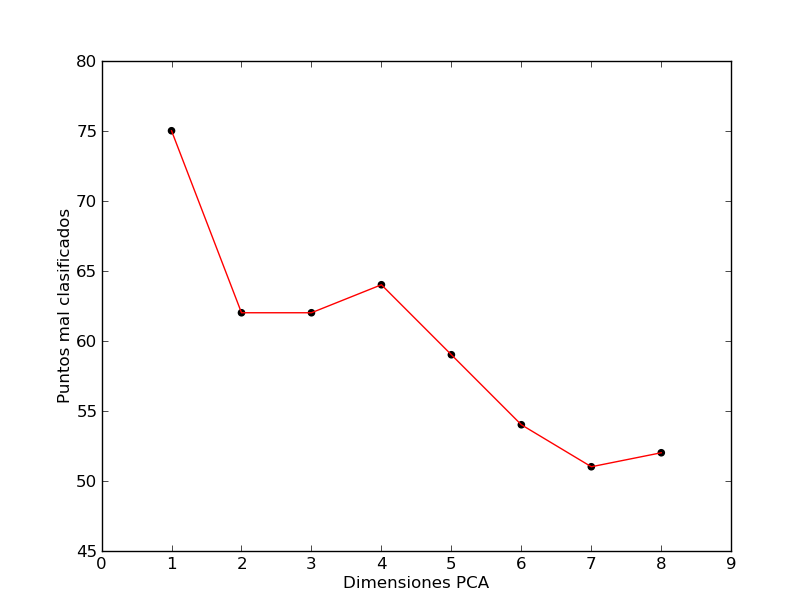
\includegraphics[width=0.8\linewidth]{images/error_pca}
        \captionof{figure}{Puntos mal clasificados vs. dimensión PCA.}
    \end{minipage}%
    \begin{minipage}{.5\textwidth}
        \centering
        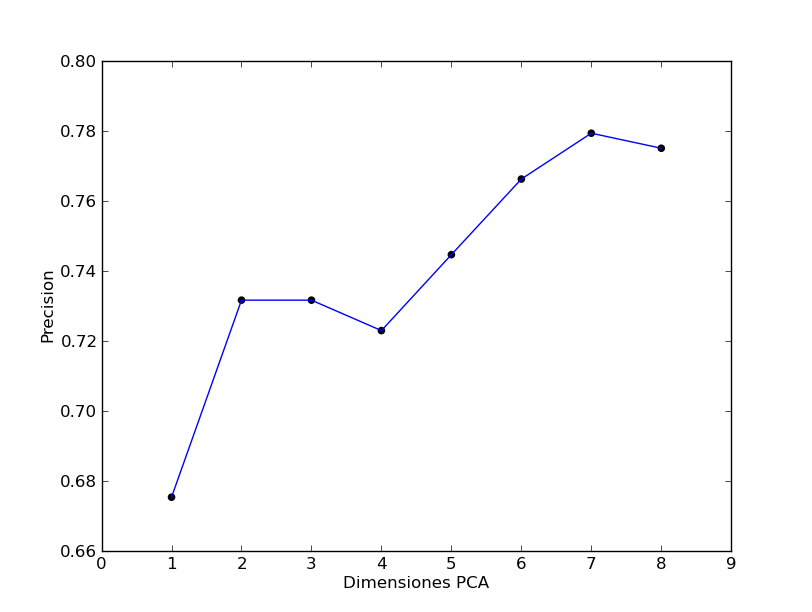
\includegraphics[width=0.8\linewidth]{images/precision_pca}
        \captionof{figure}{Precisión vs. dimensión PCA.}
    \end{minipage}
\end{figure}

Lógicamente el gráfico de la precisión es un reflejo de los puntos mal clasificados. Notar que el óptimo ocurre justamente cuando la dimensión de PCA es 7, solo una dimensión menos que el espacio original, esto implica que para este problema en específico PCA no aporta mucho al clasificador, notar que la cantidad de puntos mal clasificados solo se reduce en 1. Esto en general no se cumple, ya que en muchos casos el uso de PCA permite mejorar el rendimiento del clasificador al eliminar ruido de los datos y reducir la \textit{maldición de la dimensión}.

\subsection{PCA 1-D}
  \begin{figure}[H]
  \centering
    \begin{minipage}{.5\textwidth}
        \centering
        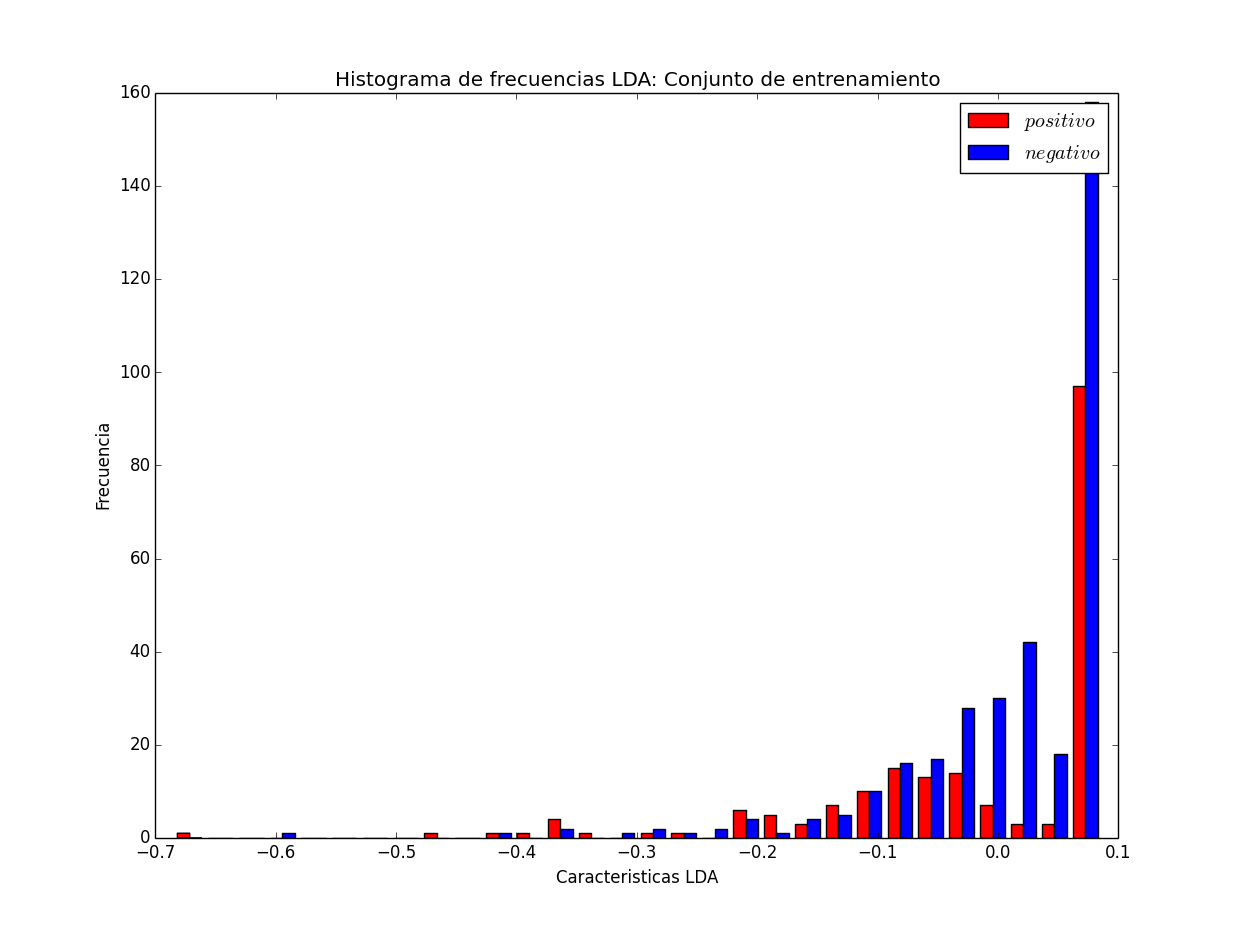
\includegraphics[width=1\linewidth]{images/Histograma_D1}
        \captionof{figure}{Histograma para 1-D}
    \end{minipage}%
    \begin{minipage}{.5\textwidth}
        \centering
        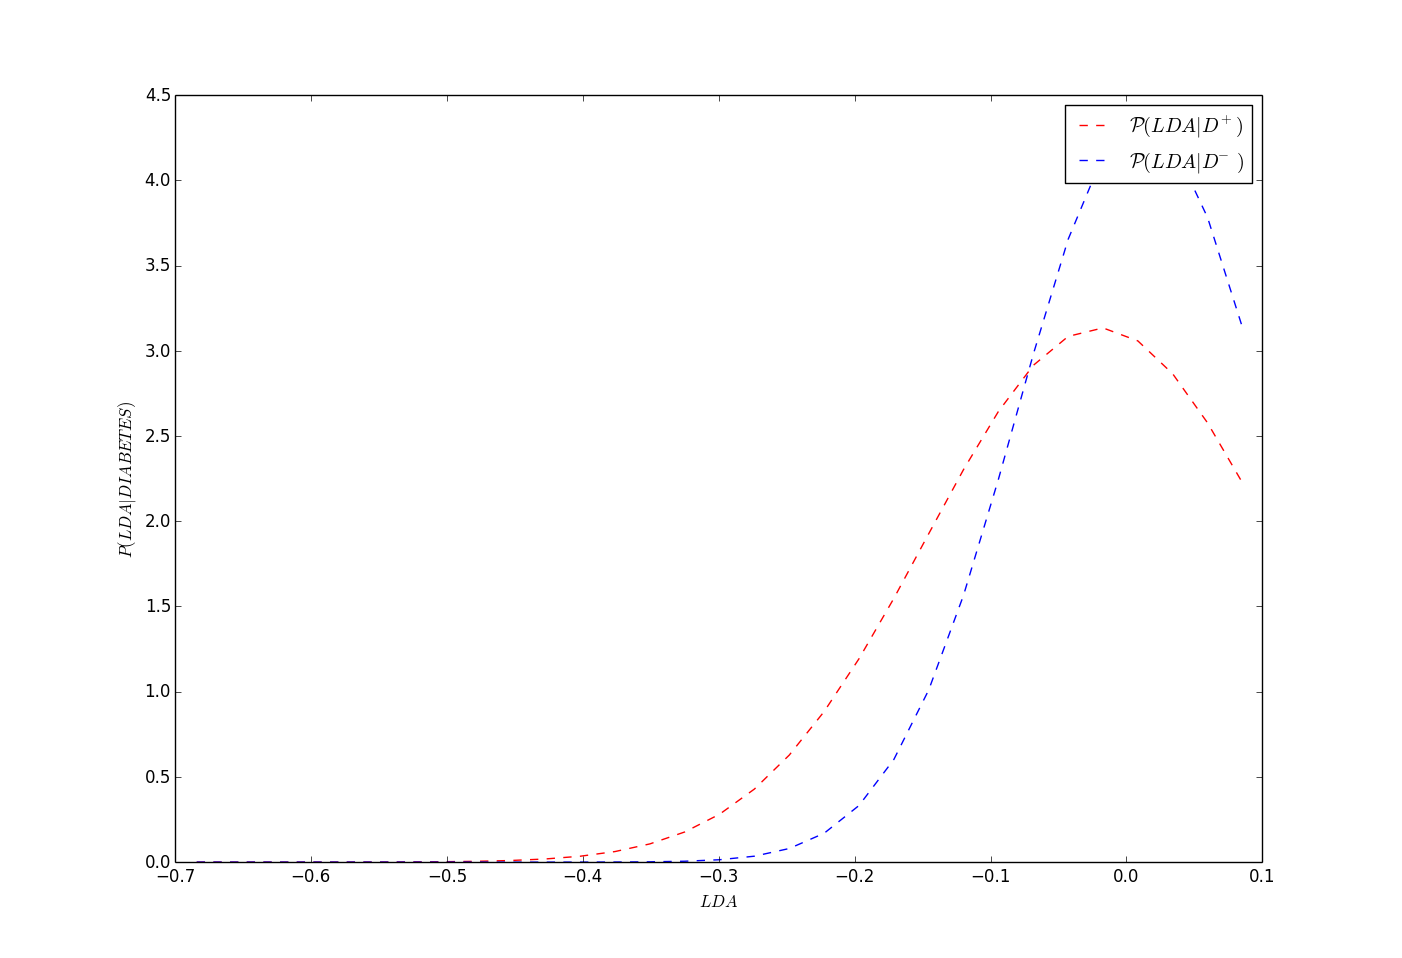
\includegraphics[width=1\linewidth]{images/PDF_D1}
        \captionof{figure}{Función de densidad de probabilidad ajustada para 1-D}
    \end{minipage}
    \begin{minipage}{.5\textwidth}
        \centering
        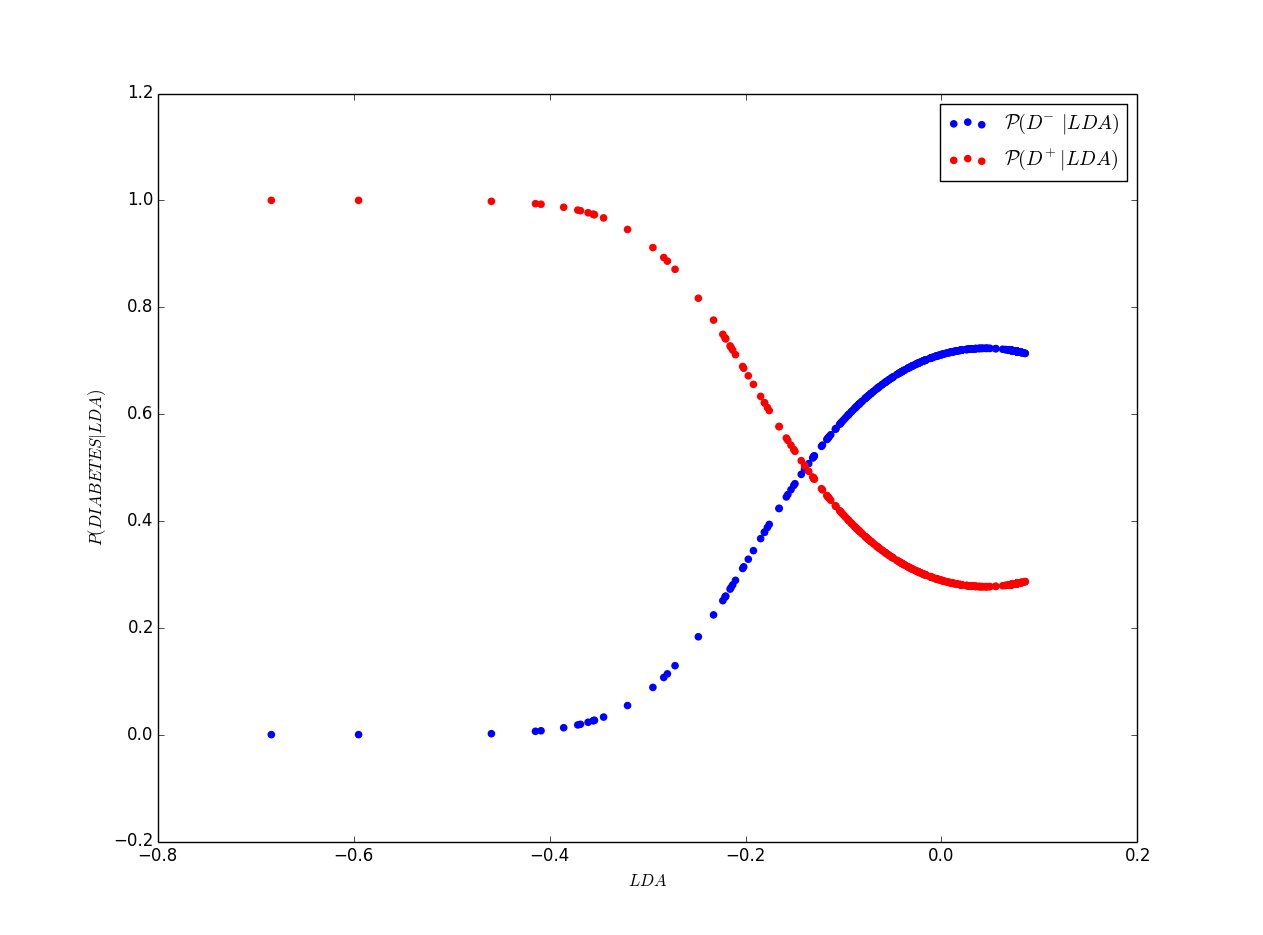
\includegraphics[width=1\linewidth]{images/CP_D1}
        \captionof{figure}{Probabilidad condicional de clase para 1-D}
    \end{minipage}
\end{figure}
Al utilizar una única dimensión para PCA se puede observar una clara pérdida de la información, esto hace que la proyección obtenida por LDA no permita clasificar de manera óptima los ejemplos de prueba. 

Se puede observar que las distribuciones se encuentran totalmente superpuestas y es prácticamente imposible distinguir entre datos positivos (diagnosticados con diabetes) y datos negativos (personas sanas). 

La posición actual del punto de intersección para este caso se encuentra con un claro sesgo a la derecha, se verá que al aumenta la dimensión este punto empieza a moverse a lo largo del eje de las abscisas hacia la izquierda, de la misma forma el centro de la distribución del valor de LDA para casos positivos se desplazará en esa dirección.

La precisión para este caso es de 67.53\%, muy detrás de todos los otros casos que superan el 70\%. Se debe destacar que a pesar del evidente problema con la superposición de igual logra clasificar más de dos tercios de los ejemplos de prueba correctamente.

\newpage

\subsection{PCA 2-D}
  \begin{figure}[H]
  \centering
    \begin{minipage}{.5\textwidth}
        \centering
        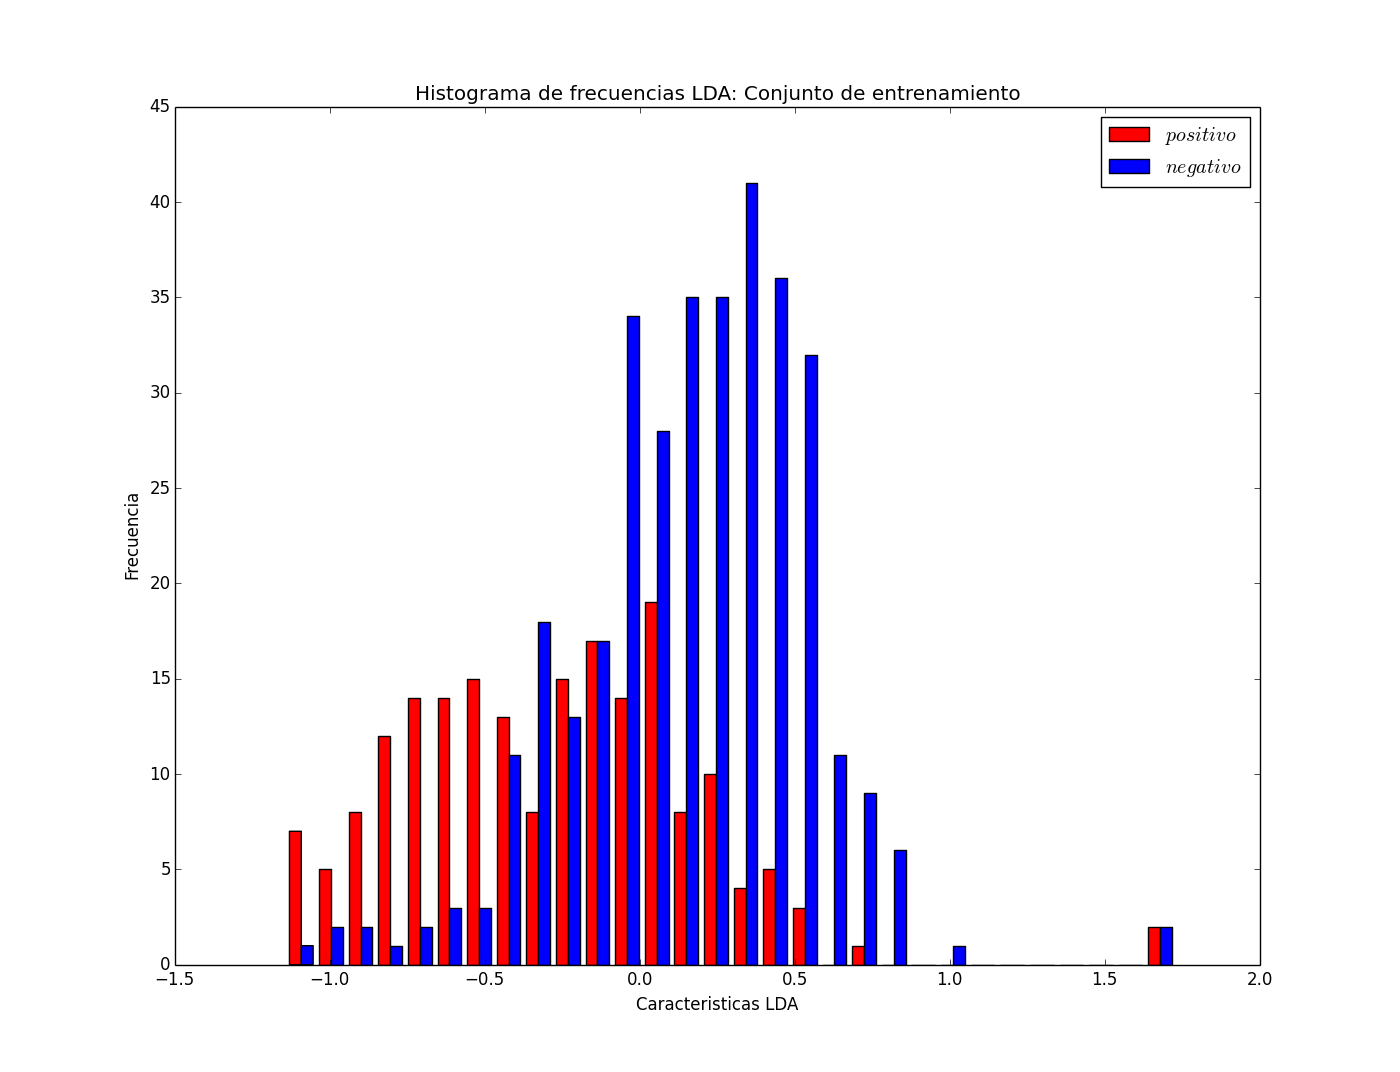
\includegraphics[width=1\linewidth]{images/Histograma_D2}
        \captionof{figure}{Histograma para 2-D}
    \end{minipage}%
    \begin{minipage}{.5\textwidth}
        \centering
        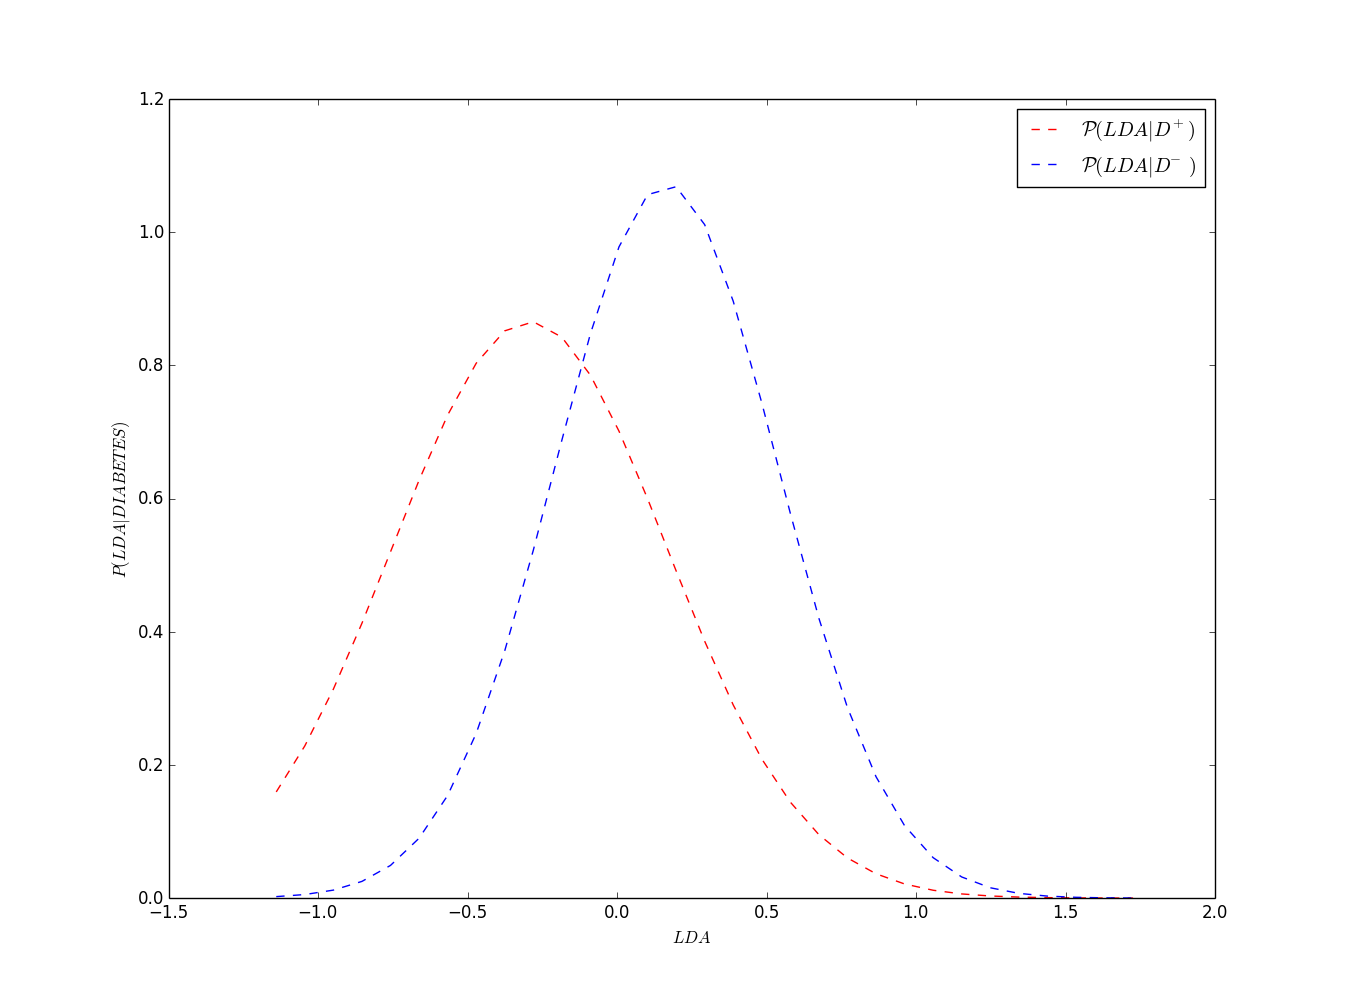
\includegraphics[width=1\linewidth]{images/PDF_D2}
        \captionof{figure}{Función de densidad de probabilidad ajustada para 2-D}
    \end{minipage}
    \begin{minipage}{.5\textwidth}
        \centering
        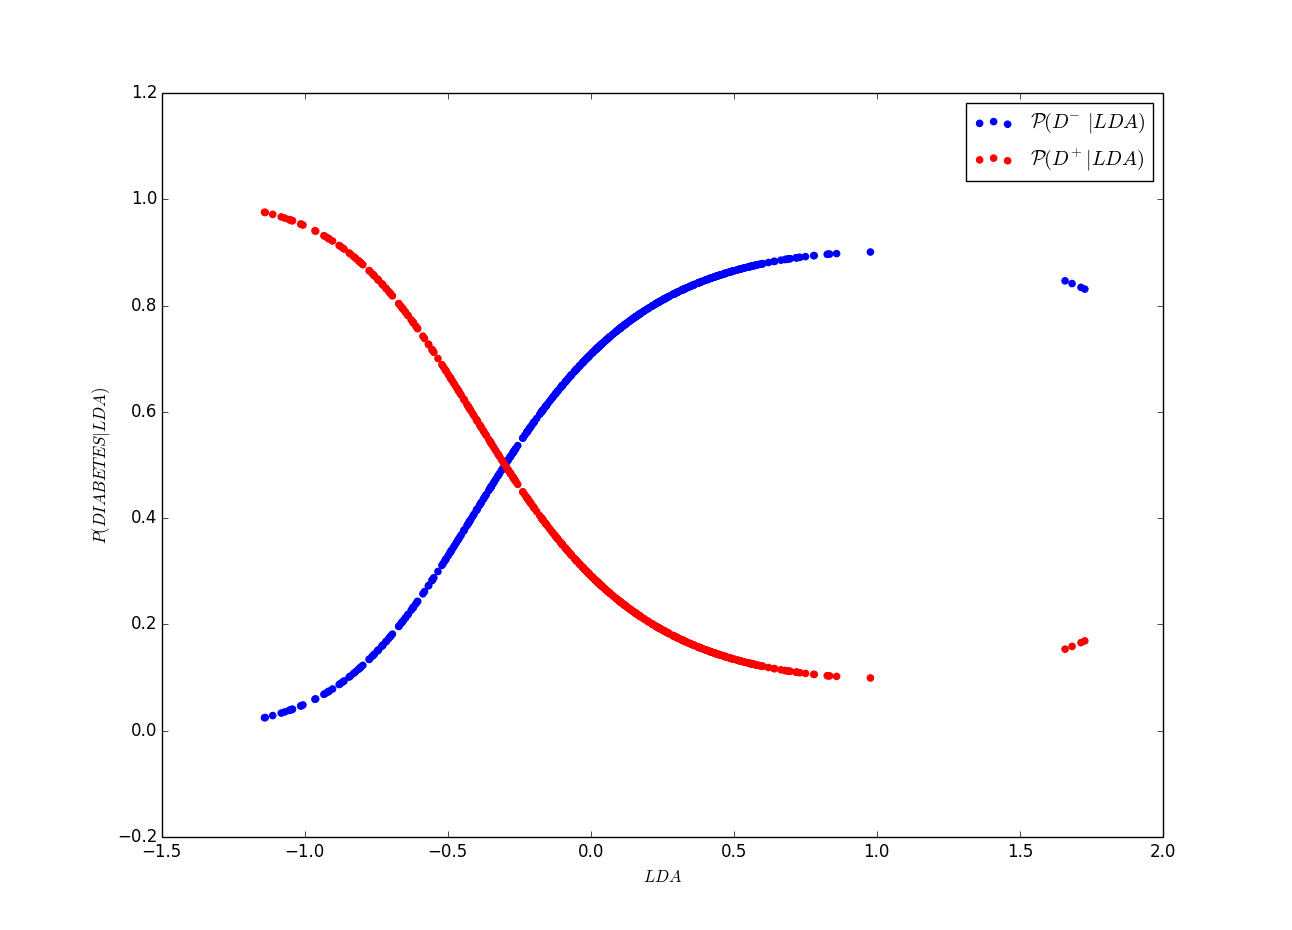
\includegraphics[width=1\linewidth]{images/CP_D2}
        \captionof{figure}{Probabilidad condicional de clase para 2-D}
    \end{minipage}
\end{figure}
Al utilizar dos dimensiones para PCA se observa una relativa mejora respecto al caso unidimensional. La pérdida de información ya no es tan alta, aunque aún está lejos de ser óptima.

Se puede observar que las distribuciones se encuentran menos superpuestas que en el caso anterior (tanto en el histograma como en el gráfico de funciones de densidad de probabilidad), esta vez es un tanto más probable distinguir entre las dos clases.

La posición actual del punto de intersección se ha desplazado hacia la izquierda, desde -0.13 que para el caso anterior hasta -0.29, a partir desde este momento el punto de intersección variará mucho, a pesar que la precisión si variará. 

La precisión para este caso es de 73.16\%, si bien no es tan óptimo como otros casos ya empieza a ser competitivo con los clasificadores que utilizaron PCA con otras dimensiones. Se debe notar que agregar esta dimensión produce el aumento más grande sobre la precisión y después se puede observar que cada dimensión aporta menos. Esto se debe a que las dimensiones son agregadas en orden descendente respecto a la variabilidad que contienen.



\newpage


\subsection{PCA 7-D}
  \begin{figure}[H]
  \centering
    \begin{minipage}{.5\textwidth}
        \centering
        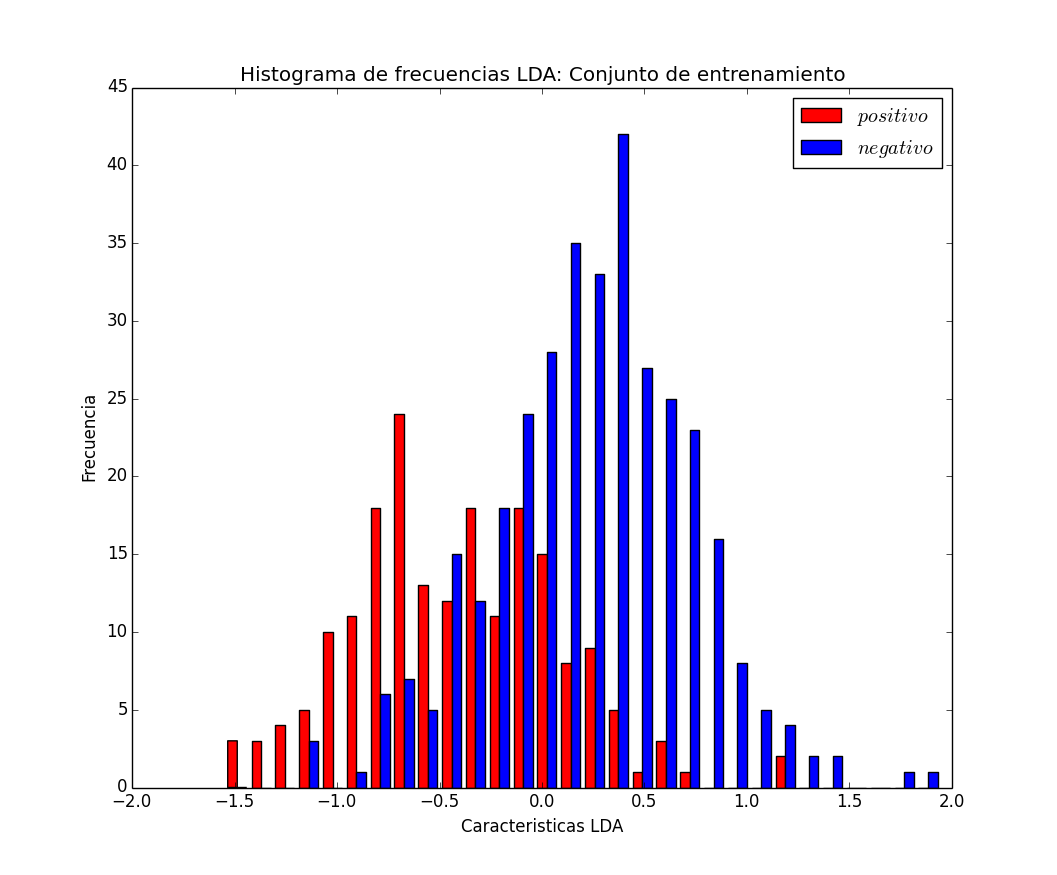
\includegraphics[width=1\linewidth]{images/Histograma_D7}
        \captionof{figure}{Histograma para 7-D}
    \end{minipage}%
    \begin{minipage}{.5\textwidth}
        \centering
        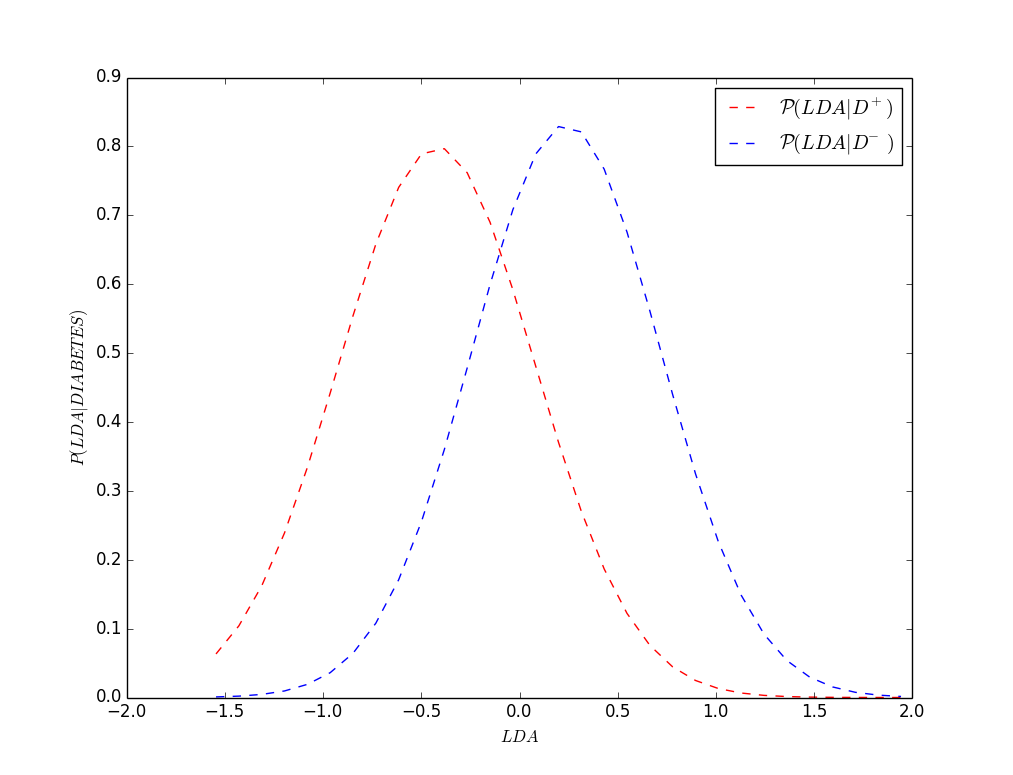
\includegraphics[width=1\linewidth]{images/PDF_D7}
        \captionof{figure}{Función de densidad de probabilidad ajustada para 7-D}
    \end{minipage}
    \begin{minipage}{.5\textwidth}
        \centering
        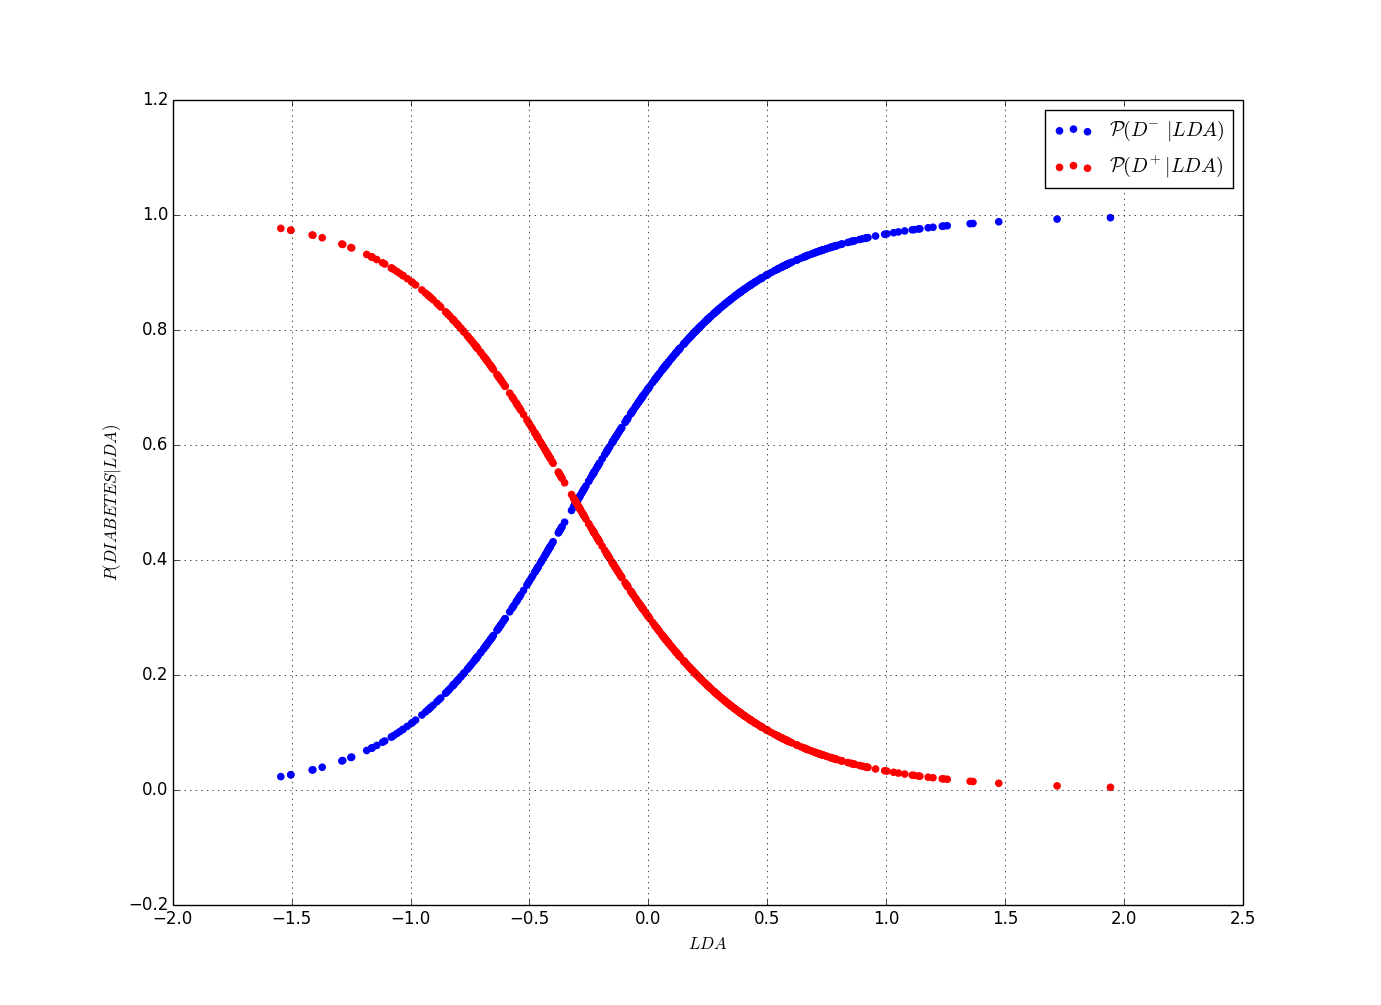
\includegraphics[width=1\linewidth]{images/CP_D7}
        \captionof{figure}{Probabilidad condicional de clase para 7-D}
    \end{minipage}
\end{figure}
Al utilizar siete dimensiones para PCA se observa que se obtiene la mejor clasificación con respecto a todas las otras dimensiones probadas. Ver Anexo 1, donde se encuentran las imágenes de los gráficos de las otras dimensiones probadas. La dimensión óptima se calculó utilizando un algoritmo que busca el clasificador que obtenga la mayor precisión de clasificación, de acuerdo a lo mostrado en la sección de implementación.

Se puede observar que las distribuciones se encuentran menos superpuestas con respecto a las otras dimensiones probadas. Desde la dimensión 5 la variabilidad no cambia demasiado, por lo que la ganancia obtenida con PCA no fue demasiada para este problema en particular.

La posición actual del punto de intersección se encuentra en -0.30

La precisión para este caso es de 77.92\%,

\newpage

%-----------------------------------------------------------------------------------
% SECTION 5
%----------------------------------------------------------------------------------------
\newpage
\section{Conclusiones}
Se ha completado satisfactoriamente el objetivo del taller II que correspondía a construir un diagnosticador de diabetes utilizando PCA, LDA y un clasificador Gaussiano basado en Naïve Bayes. Este trabajo ha contribuido en mejorar el entendimiento de las técnicas de predicciones aprendidas en clases mediante su uso e implementación. Además, ha permitido profundizar el conocimiento adquirido en cátedra, ya que el desarrollo del taller ha requerido de una extensa recopilación bibliográfica del tema además de estudiar las posibles implementaciones del clasificador bayesiano.

Se ha mostrado además la clara diferencia que existe en la precisión entregada por el clasificador dependiendo de la cantidad de componentes que hayan sido usados con PCA, se ha comprobado empirícamente que la mejor precisión se obtiene con 7 dimensiones. Además se ha mencionado la diferencia que produce el salto desde 1 dimensión a 2 dimensiones para PCA sobre la precisión del método. Cabe destacar que después de agregar la 2da dimensión el rendimiento del clasificador crece lentamente, esto debido a que cada dimensión contiene cada vez menor variabilidad, produciéndose un efecto de rendimientos decrecientes a medida que se aumentaba la cantidad de dimensiones, después del óptimo la calidad del clasificador empezó a disminuir.

Se debe mencionar que si para PCA se utiliza una única dimensión el rendimento del algoritmo es bajo respecto a los demás casos, esto debido a que si se hace una reducción solo sobre la primera componente principal se pierde mucha información contenida en otras dimensiones del problema.

Los datos utilizados para el desarrollo de este taller presentaron la particularidad que PCA no redujo mucho la cantidad de dimensiones, esto no ocurre en el caso general, donde el uso de PCA permite reducir en gran medida la dimensión de los datos al eliminar ruido e información redundante. En este caso la dimensión solo se redujo de 8 a 7, un cambio no muy significativo y que solo aportó en un ejemplo más clasificado correctamente. En otros casos el aporte de PCA puede ser significativo y permitir grandes mejoras del rendimiento, pues permite reducir la \textit{maldición de la dimensión}.

Una propuesta interesante sería probar la implementación realizada con datos de otro problema de mayores dimensiones en función de observar si PCA produce un cambio significativo. También sería interesante generalizar el código implementado a problemas con más de dos clases, ya que la implementación actual del clasificador bayesiano propio solo admite problemas de clasificación binaria, a diferencia de la implementación de la librería \textit{scikit-learn} que admite problemas de clasificación $n$-arios.

El uso de la librería \textit{scikit-learn} en el desarrollo del taller facilitó bastante la implementación, ya que esta contenía todos los métodos utilizados ya implementados. Lamentablemente la librería no se pudo hacer funcionar en Windows, por lo que para evitar problemas se realizó toda la implementación en un ambiente Linux.

Por último, queda por mencionar los problemas encontrados durante el desarrollo del taller, a decir, la implementación propia del clasificador bayesiano, esto debido a que la bibliografía referenciada contenía diferentes métodos para determinar la clase a que pertenecía una instancia de los datos. Si bien todos estos métodos son equivalentes, hubo problema con la implementación de las fórmulas debido a ciertas incongruencias encontradas en las fuentes, una vez se tuvo las fórmulas correctas el clasificador funcionó de manera idéntica al clasificador de la librería \textit{scikit-learn}.

%----------------------------------------------------------------------------------------
% BIBLIOGRAPHY
%----------------------------------------------------------------------------------------

\newpage
\bibliographystyle{apalike}

%Se presenta la bibliografía utilizada para el desarrollo del taller, desde los ejemplos de código utilizados, los fundamentos teóricos de los algoritmos.

\begin{thebibliography}{10} % 10 the total number of references
    % Libro guía
    \bibitem{1} S. Russell {\em Artificial Intelligence.} 2010: A Modern Approach.

    \bibitem{2} Peña, D. (2002). {\em Análisis de datos multivariantes (Vol. 24)}. Madrid: McGraw-Hill.

    %Experiencias
    \bibitem{3} Sridhar Mahadevan. {\em Linear Classification Models}. Recuperado Julio 19, 2014, desde http://edlab-www.cs.umass.edu/cs589/2010-lectures/bayesian-classification.pdf
    
    %Problema del laberinto
    \bibitem{4} {\em Código fuente scikit-learn}. Recuperado Julio 19, 2014, desde https://github.com/scikit-learn/scikit-learn/blob/master/sklearn/naive\_bayes.py
    
    \bibitem{5} {\em Linear Discriminant Analysis - Part I}. Recuperado Julio 19, 2014, desde https://onlinecourses.science.psu.edu/stat557/book/export/html/35
    
    \bibitem{6} Jia Li. {\em  Linear Discriminant Analysis}. Recuperado Julio 19, 2014, desde http://sites.stat.psu.edu/~jiali/course/stat597e/notes2/lda.pdf
    
    \bibitem{7} Iyad Batal, {\em Principal Component Analysis}. http://people.cs.pitt.edu/~iyad/PCA.pdf

    \bibitem{8} Meng Xu, {\em An intuitive explanation of PCA}. http://mengnote.blogspot.com/2013/05/an-intuitive-explanation-of-pca.html

    \bibitem{9} Bekios-Calfa, J., Buenaposada, J. M., \& Baumela, L. (2011). {\em Revisiting linear discriminant techniques in gender recognition}. Pattern Analysis and Machine Intelligence, IEEE Transactions on, 33(4), 858-864.
    
    \bibitem{10} Vincent Sigillito. (1990). {\em Pima Indians Diabetes Data Set}, The Johns Hopkins University. Recuperado Julio 19, 2014, desde https://archive.ics.uci.edu/ml/datasets/Pima+Indians+Diabetes
\end{thebibliography}

\newpage
\begin{appendices}
  \renewcommand\thetable{\thesection\arabic{table}}
  \renewcommand\thefigure{\thesection\arabic{figure}}

  \section{Gráficos Restantes} 

  \begin{figure}[H]
  \centering
    \begin{minipage}{.5\textwidth}
        \centering
        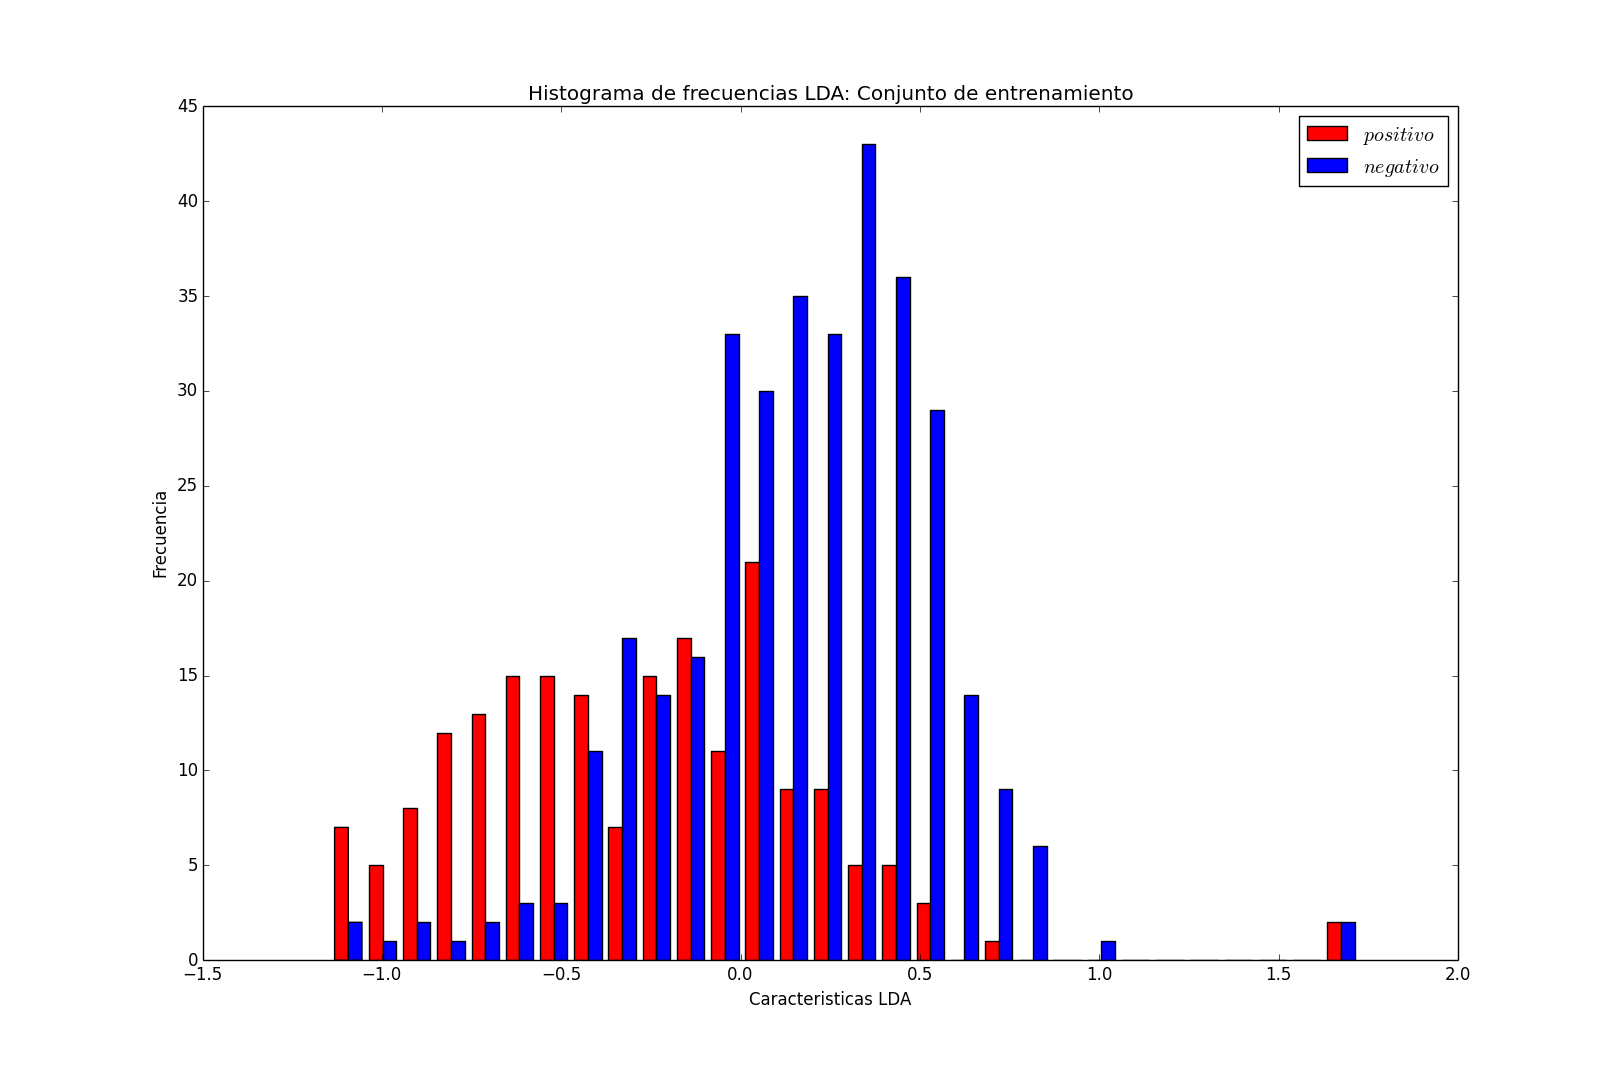
\includegraphics[width=1\linewidth]{images/Histograma_D3}
        \captionof{figure}{Histograma para 3-D}
    \end{minipage}%
    \begin{minipage}{.5\textwidth}
        \centering
        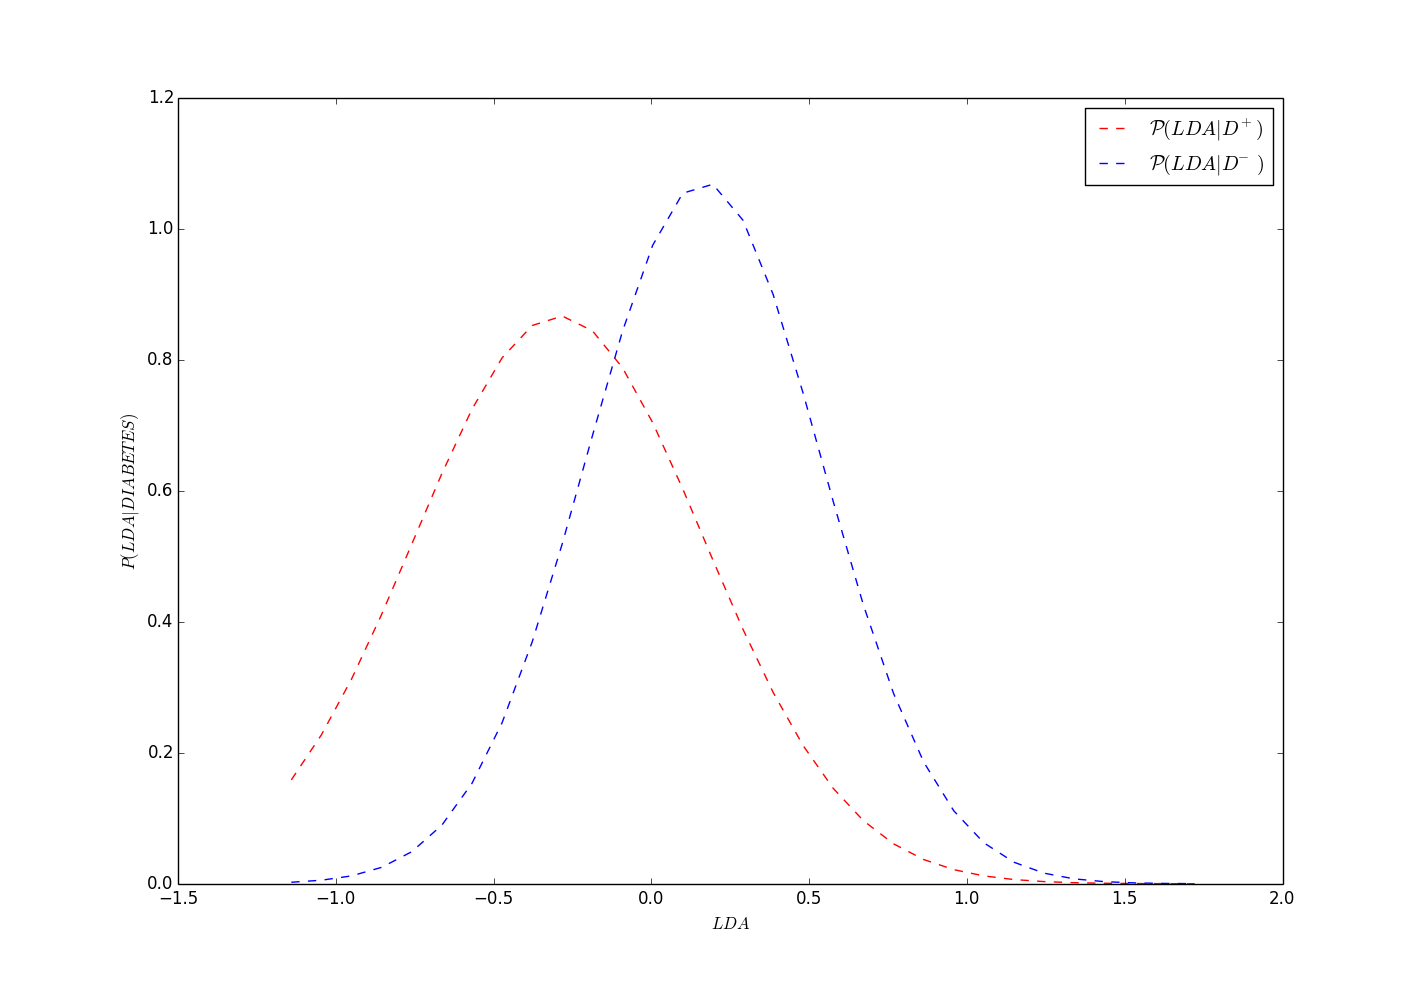
\includegraphics[width=1\linewidth]{images/PDF_D3}
        \captionof{figure}{Función de densidad de probabilidad ajustada para 3-D}
    \end{minipage}
\end{figure}

  \begin{figure}[H]
  \centering
    \begin{minipage}{.5\textwidth}
        \centering
        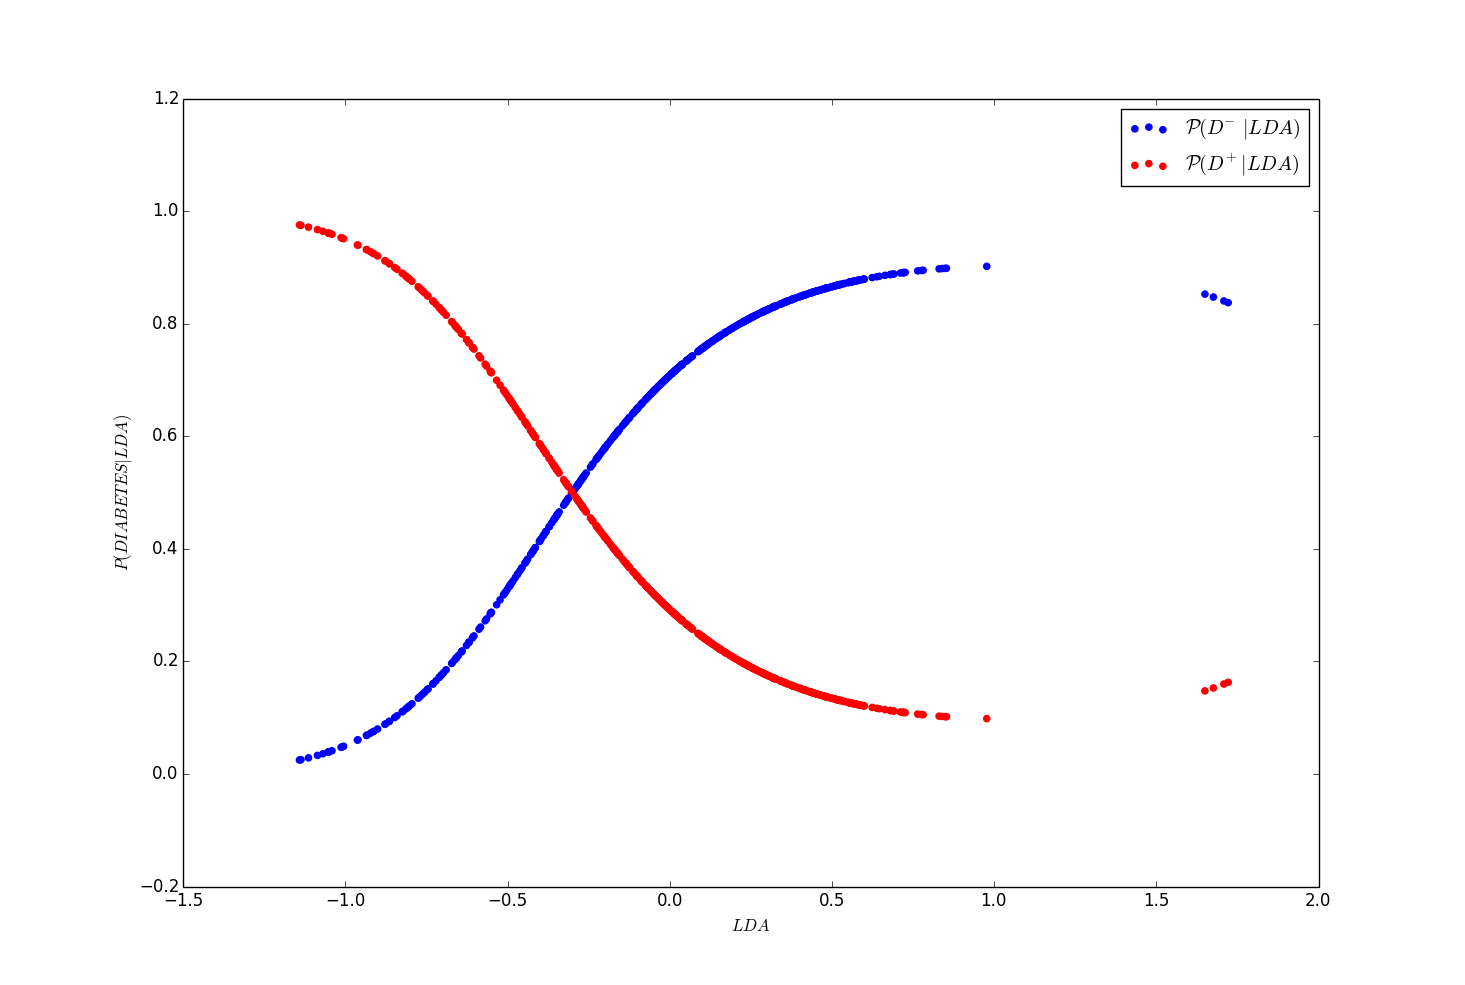
\includegraphics[width=1\linewidth]{images/CP_D3}
        \captionof{figure}{Probabilidad condicional de clase para 3-D}
    \end{minipage}%
    \begin{minipage}{.5\textwidth}
        \centering
        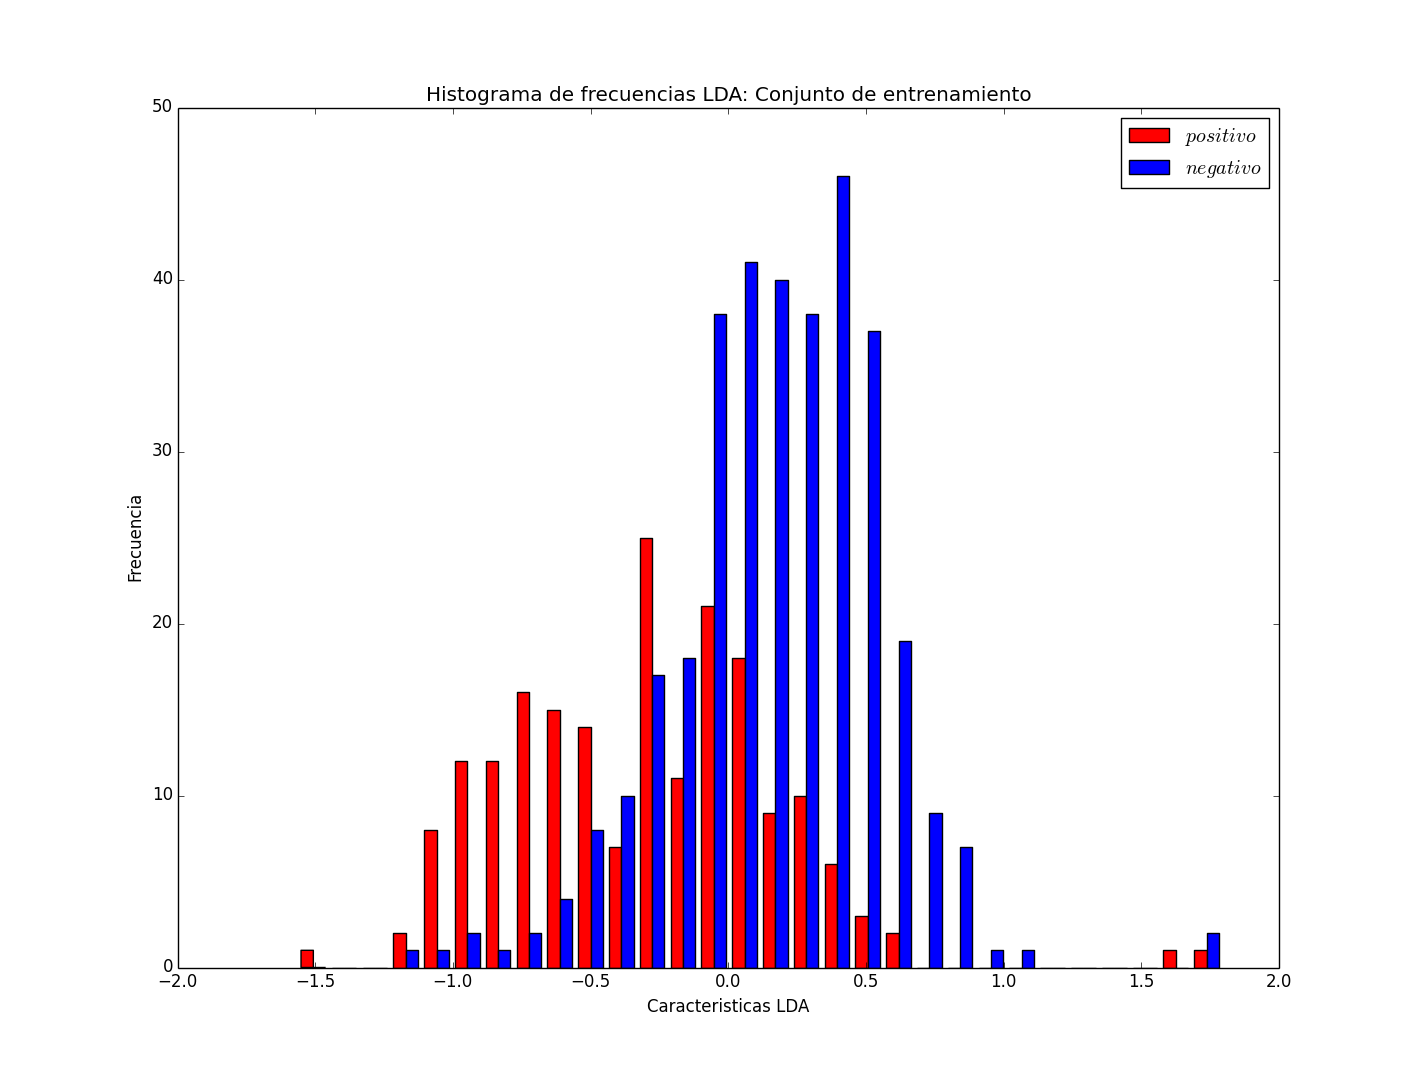
\includegraphics[width=1\linewidth]{images/Histograma_D4}
        \captionof{figure}{Histograma para 4-D}
    \end{minipage}
\end{figure}

  \begin{figure}[H]
  \centering
    \begin{minipage}{.5\textwidth}
        \centering
        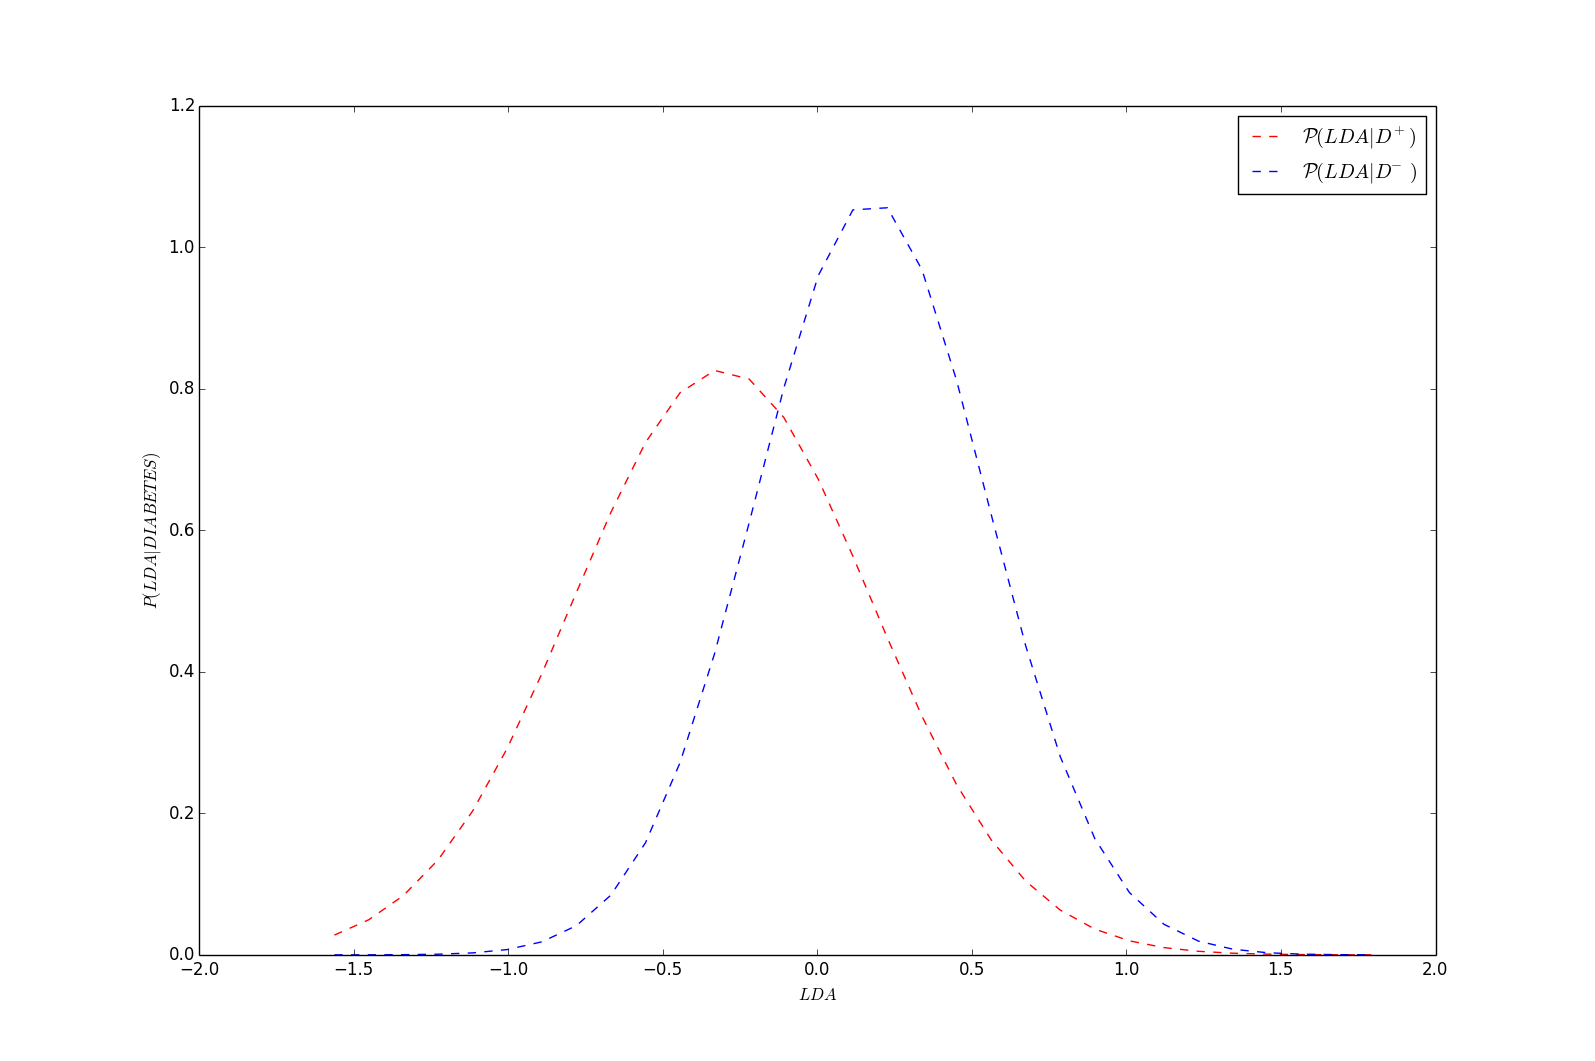
\includegraphics[width=1\linewidth]{images/PDF_D4}
        \captionof{figure}{Función de densidad de probabilidad ajustada para 4-D}
    \end{minipage}%
    \begin{minipage}{.5\textwidth}
        \centering
        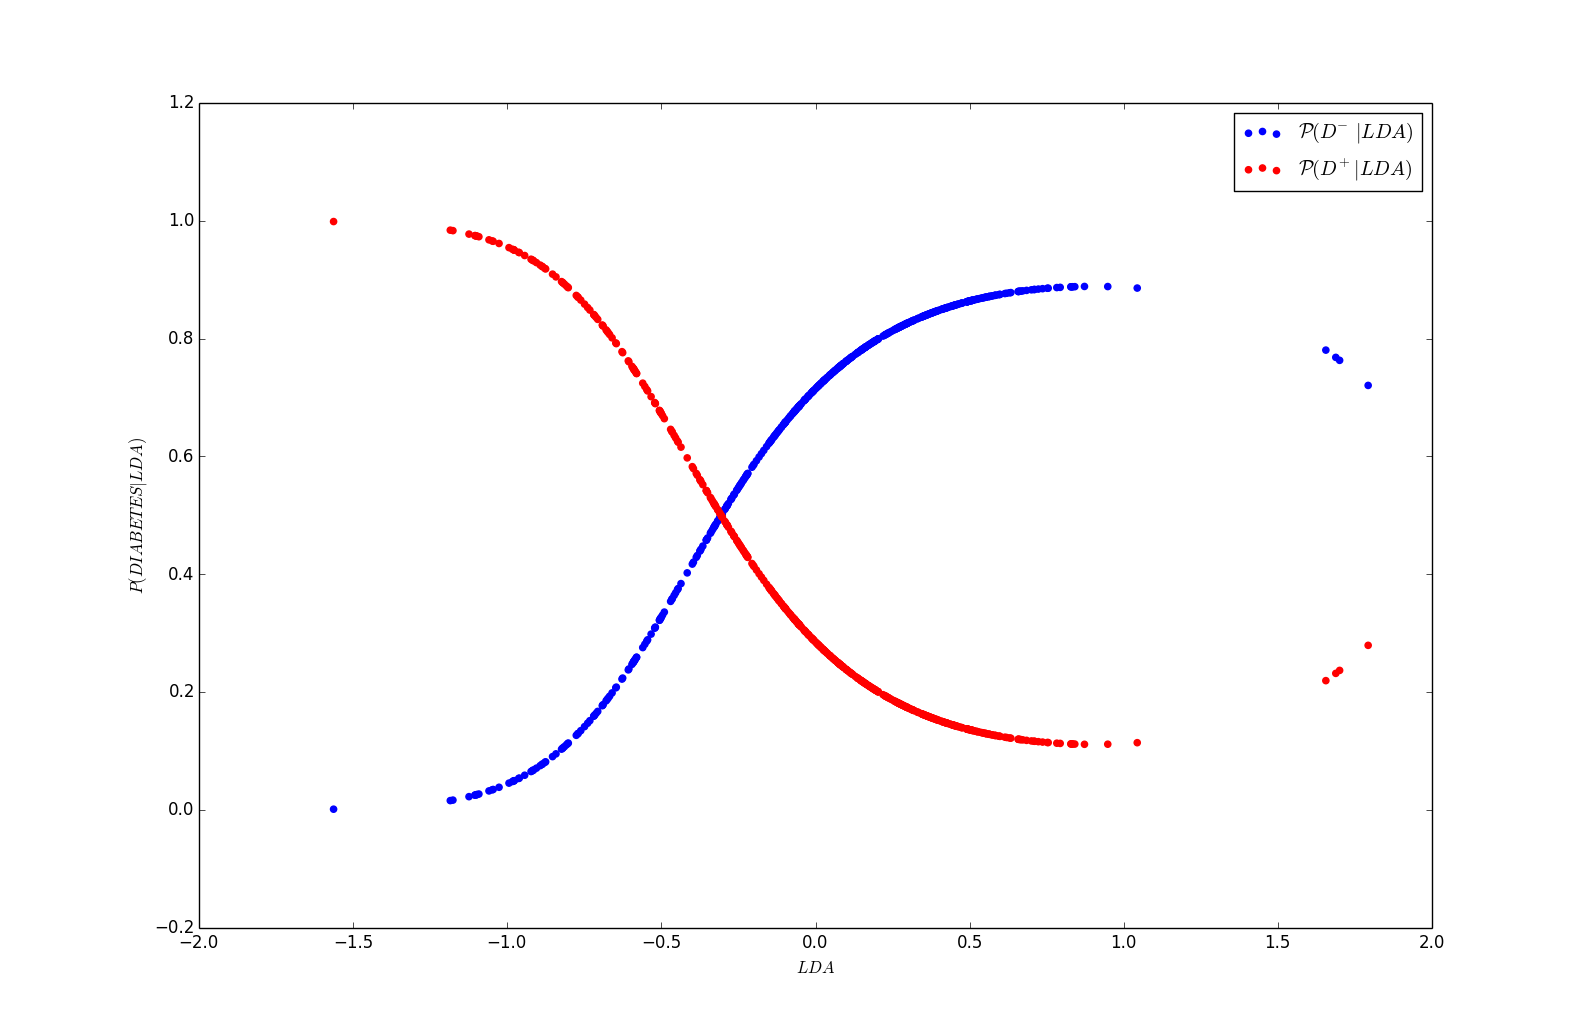
\includegraphics[width=1\linewidth]{images/CP_D4}
        \captionof{figure}{Probabilidad condicional de clase para 4-D}
    \end{minipage}
\end{figure}

  \begin{figure}[H]
  \centering
    \begin{minipage}{.5\textwidth}
        \centering
        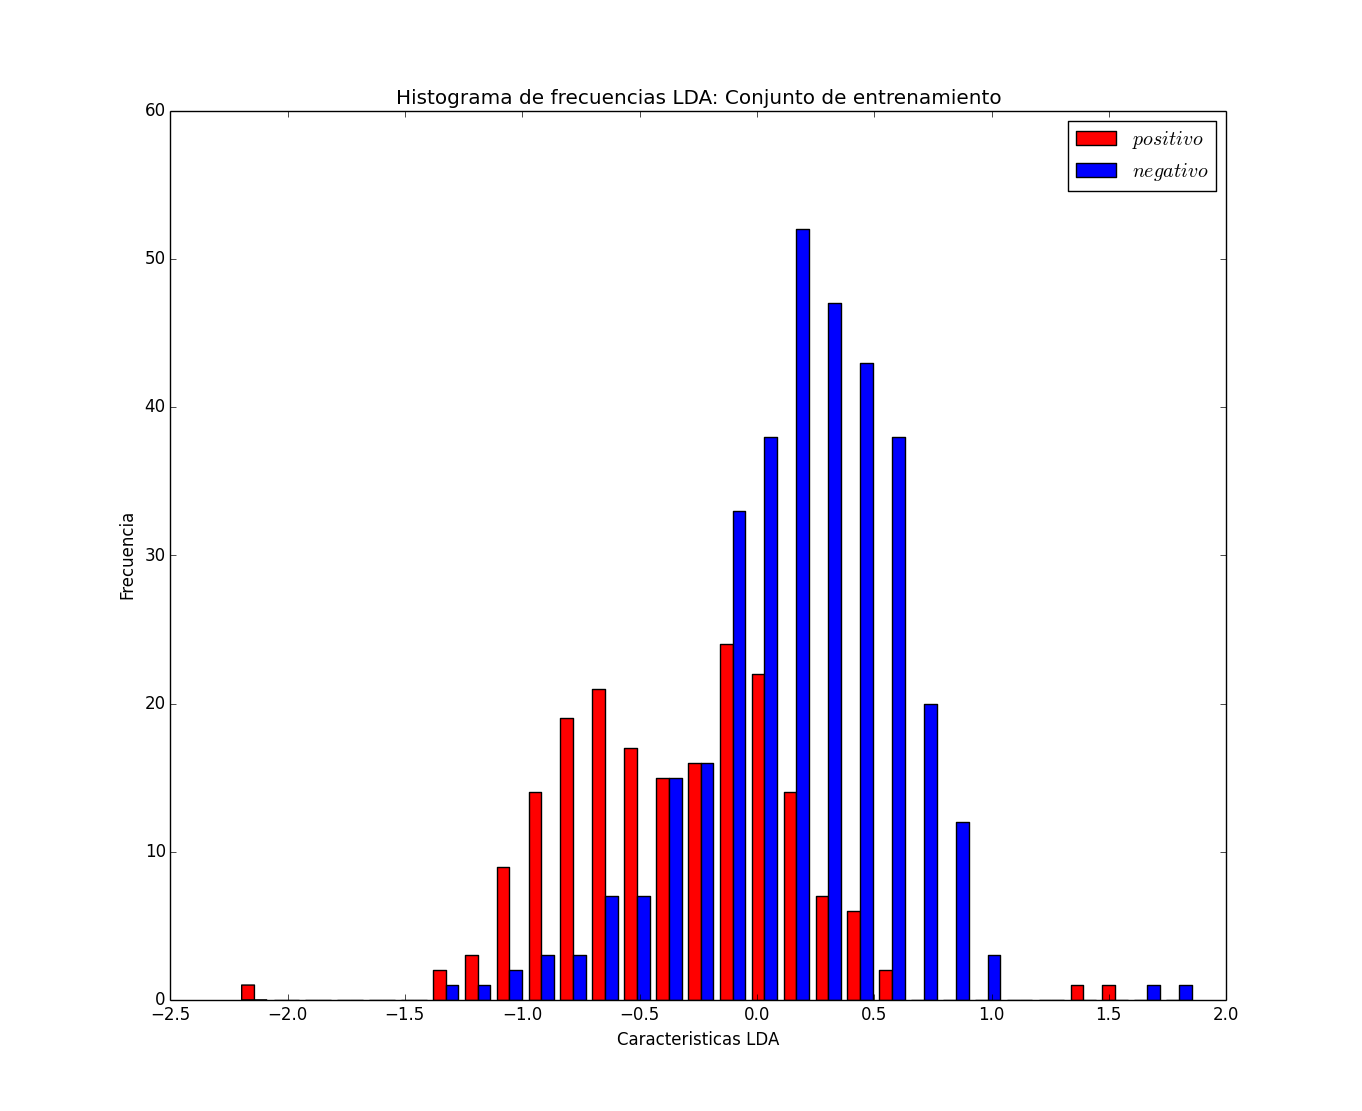
\includegraphics[width=1\linewidth]{images/Histograma_D5}
        \captionof{figure}{Histograma para 5-D}
    \end{minipage}%
    \begin{minipage}{.5\textwidth}
        \centering
        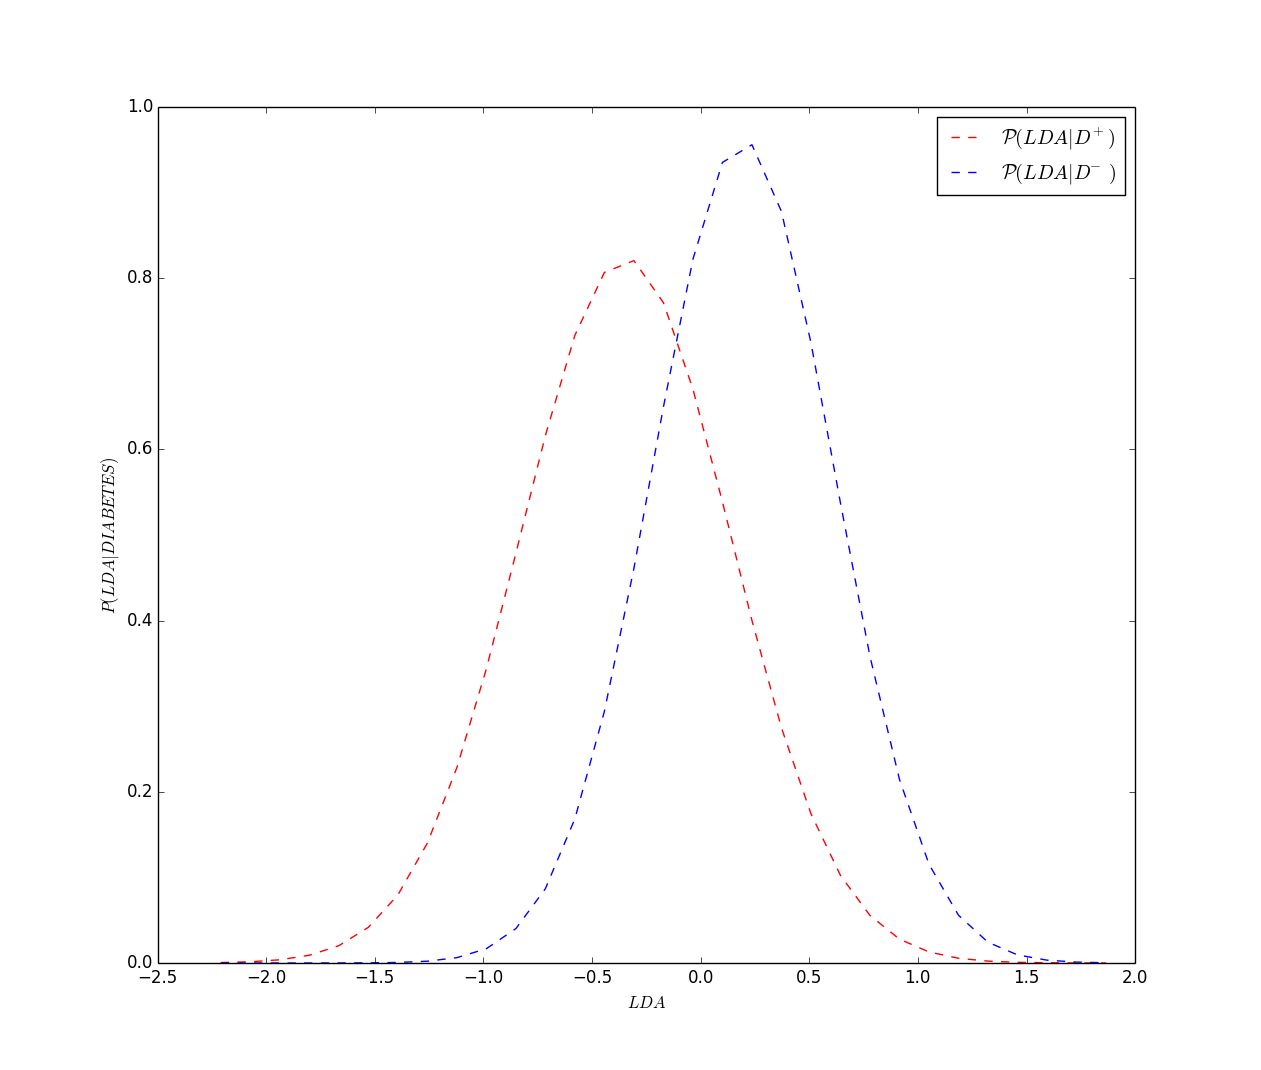
\includegraphics[width=1\linewidth]{images/PDF_D5}
        \captionof{figure}{Función de densidad de probabilidad ajustada para 5-D}
    \end{minipage}
\end{figure}

  \begin{figure}[H]
  \centering
    \begin{minipage}{.5\textwidth}
        \centering
        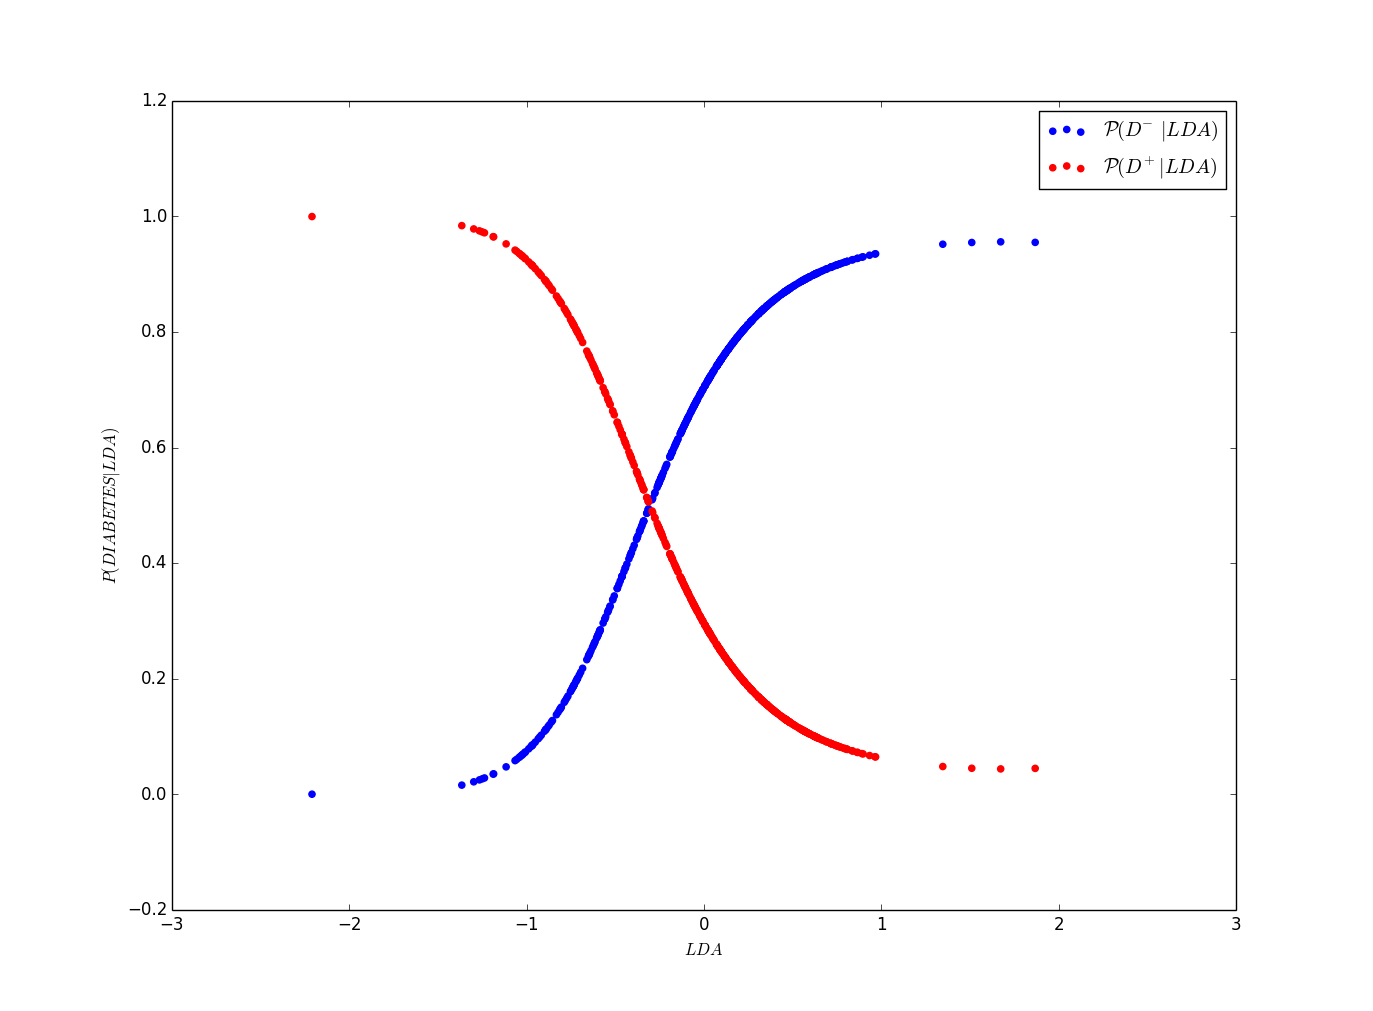
\includegraphics[width=1\linewidth]{images/CP_D5}
        \captionof{figure}{Probabilidad condicional de clase para 5-D}
    \end{minipage}%
    \begin{minipage}{.5\textwidth}
        \centering
        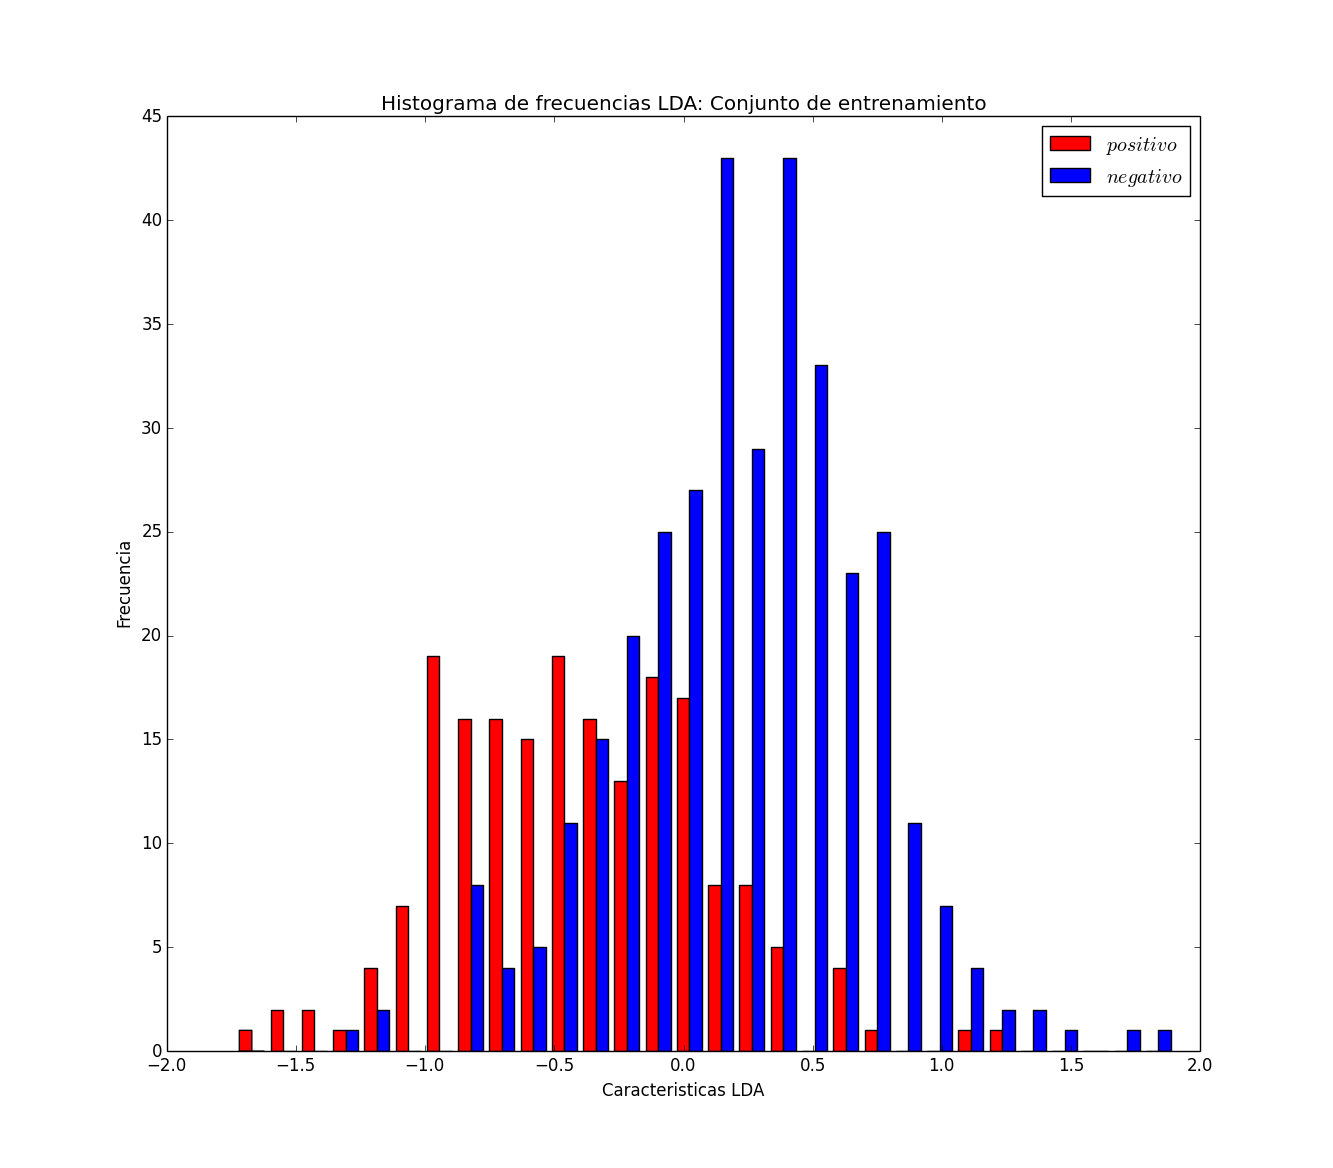
\includegraphics[width=1\linewidth]{images/Histograma_D6}
        \captionof{figure}{Histograma para 6-D}
    \end{minipage}
\end{figure}

\begin{figure}[H]
\centering
    \begin{minipage}{.5\textwidth}
        \centering
        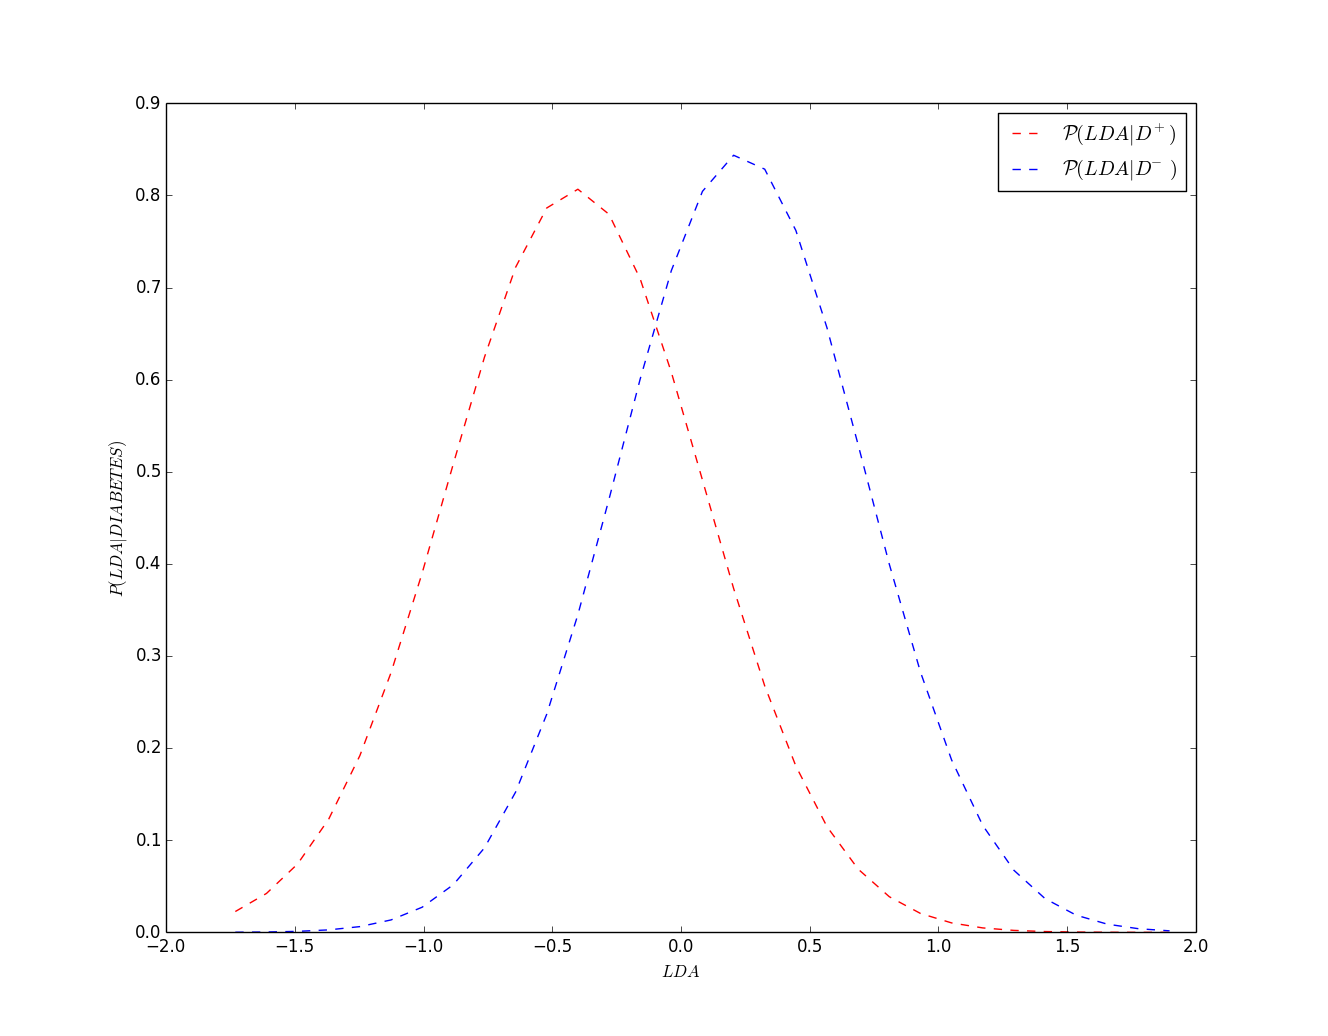
\includegraphics[width=1\linewidth]{images/PDF_D6}
        \captionof{figure}{Función de densidad de probabilidad ajustada para 6-D}
    \end{minipage}%
    \begin{minipage}{.5\textwidth}
        \centering
        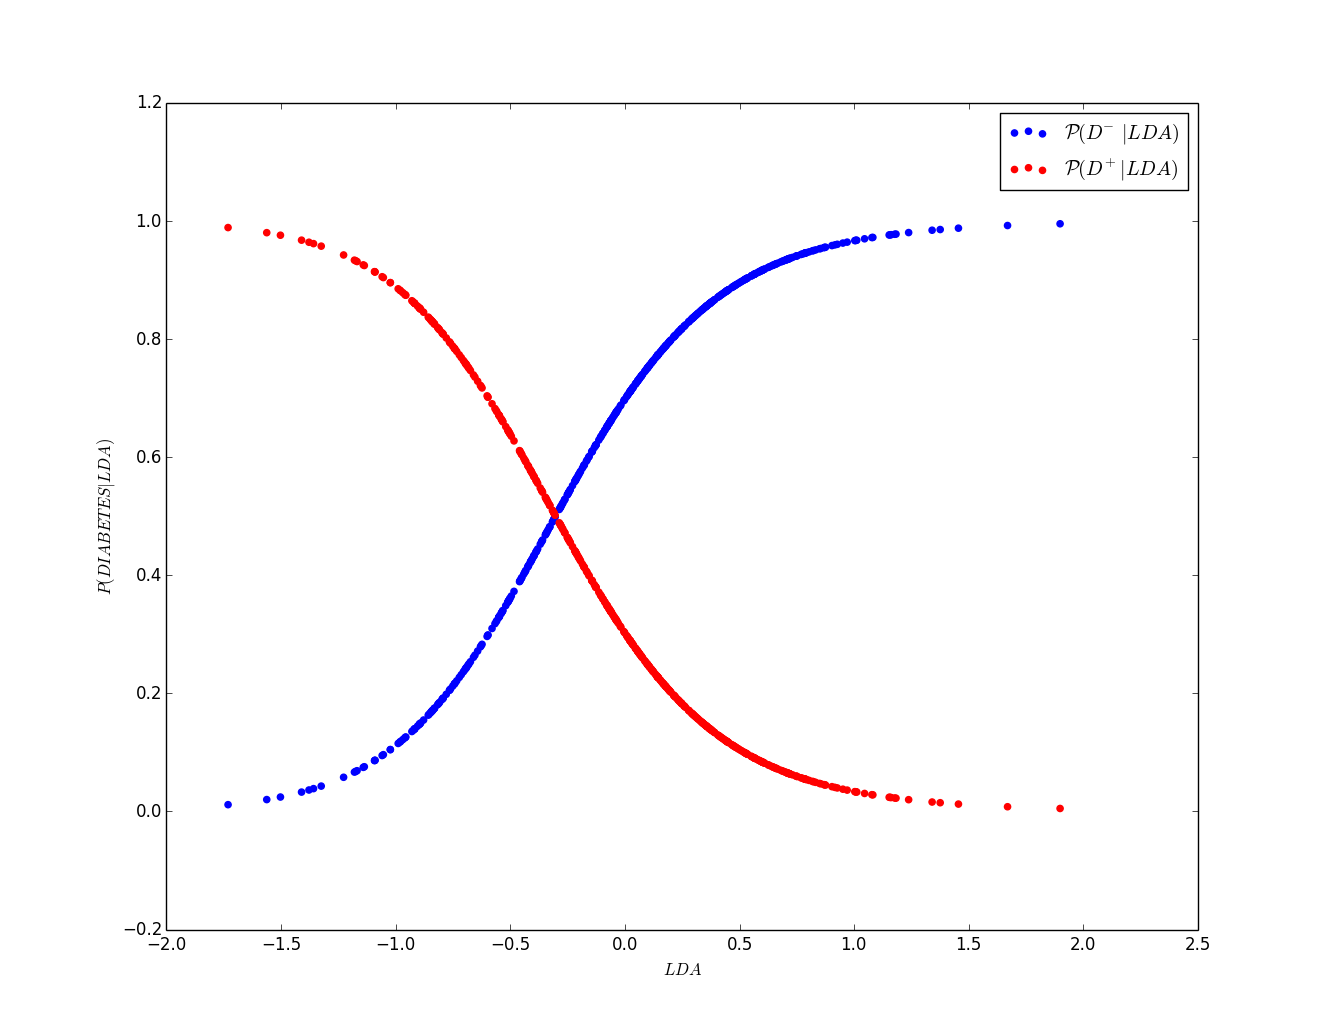
\includegraphics[width=1\linewidth]{images/CP_D6}
        \captionof{figure}{Probabilidad condicional de clase para 6-D}
    \end{minipage}
\end{figure}
\begin{figure}
\centering
    \begin{minipage}{.5\textwidth}
        \centering
        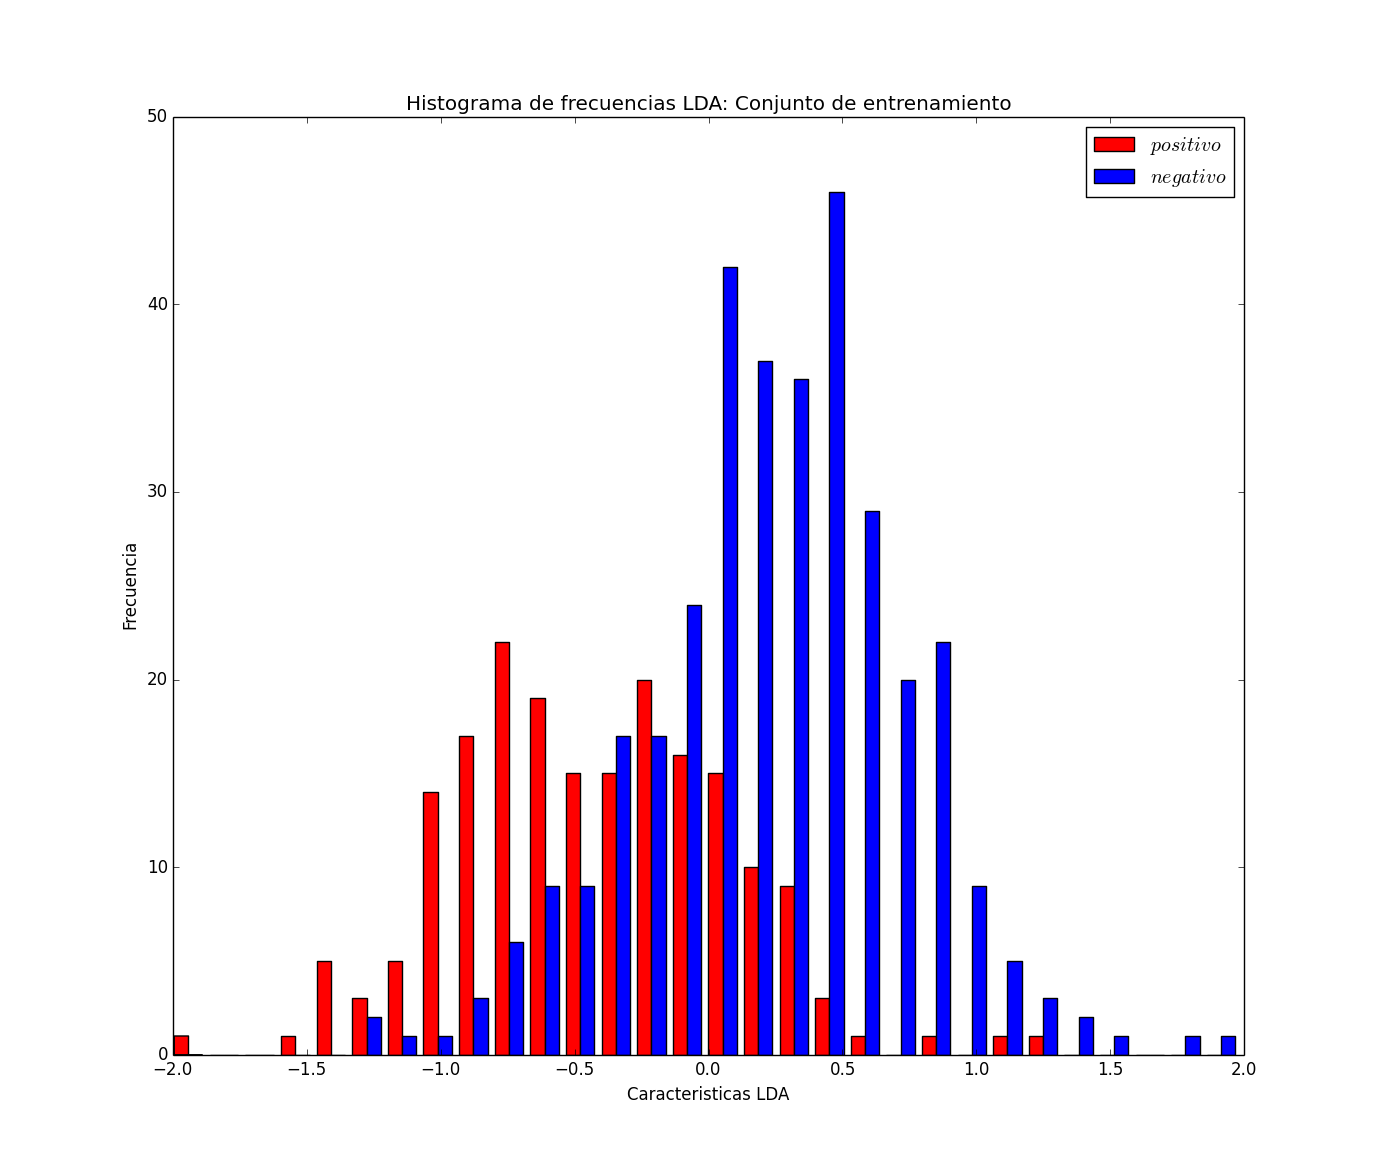
\includegraphics[width=1\linewidth]{images/Histograma_D8}
        \captionof{figure}{Histograma para 8-D}
    \end{minipage}%
    \begin{minipage}{.5\textwidth}
        \centering
        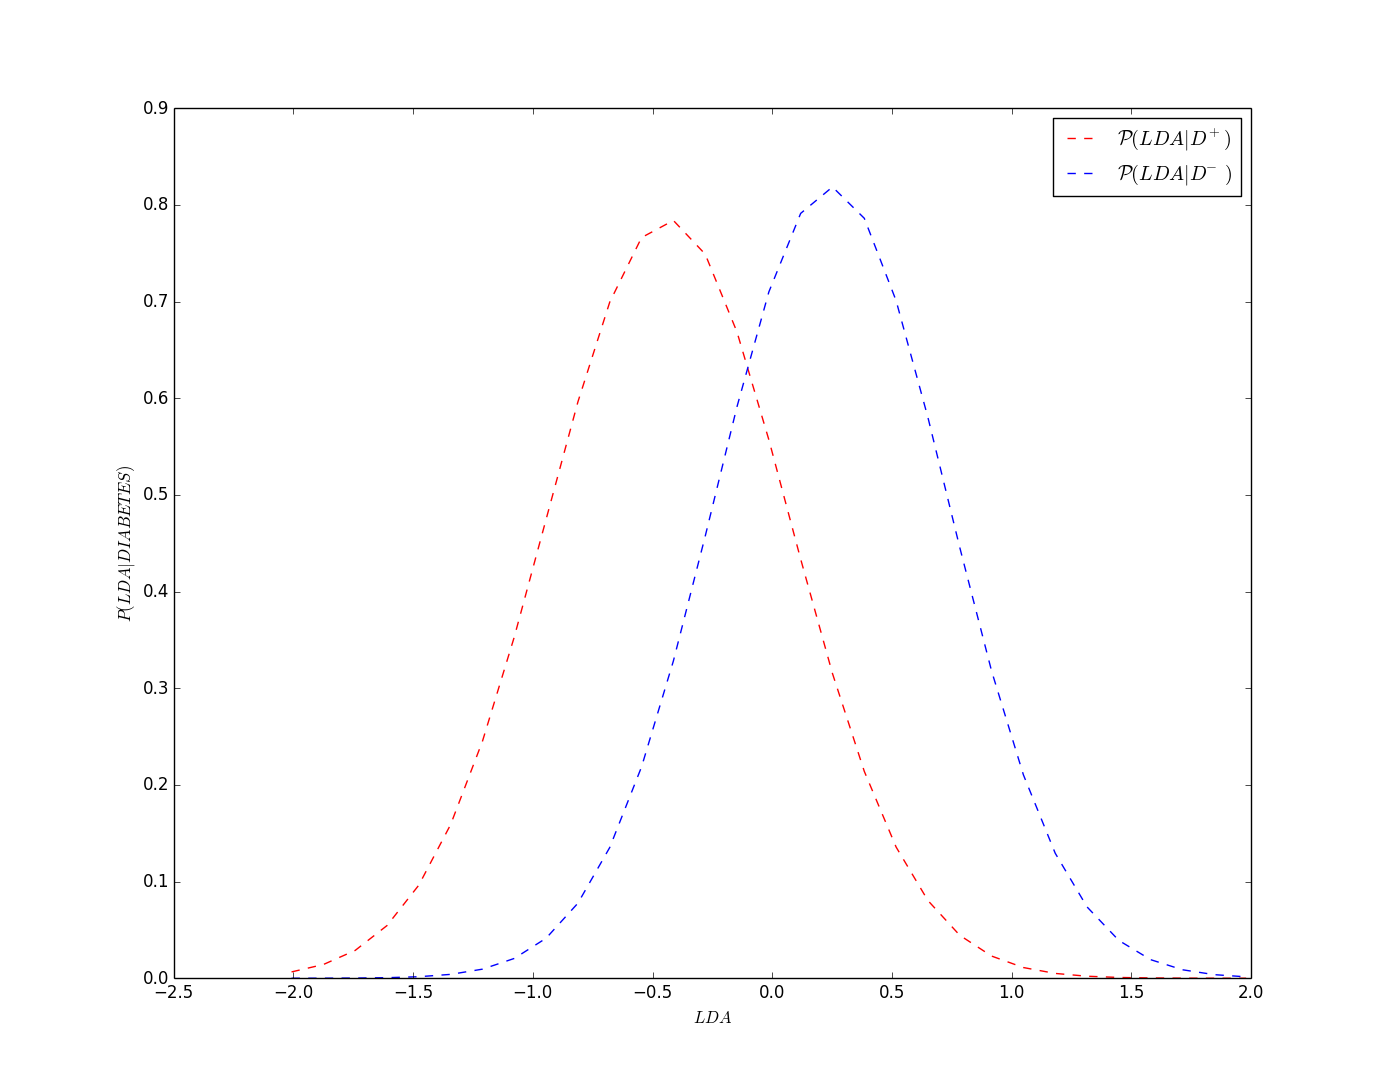
\includegraphics[width=1\linewidth]{images/PDF_D8}
        \captionof{figure}{Función de densidad de probabilidad ajustada para 8-D}
    \end{minipage}
    \begin{minipage}{.5\textwidth}
        \centering
        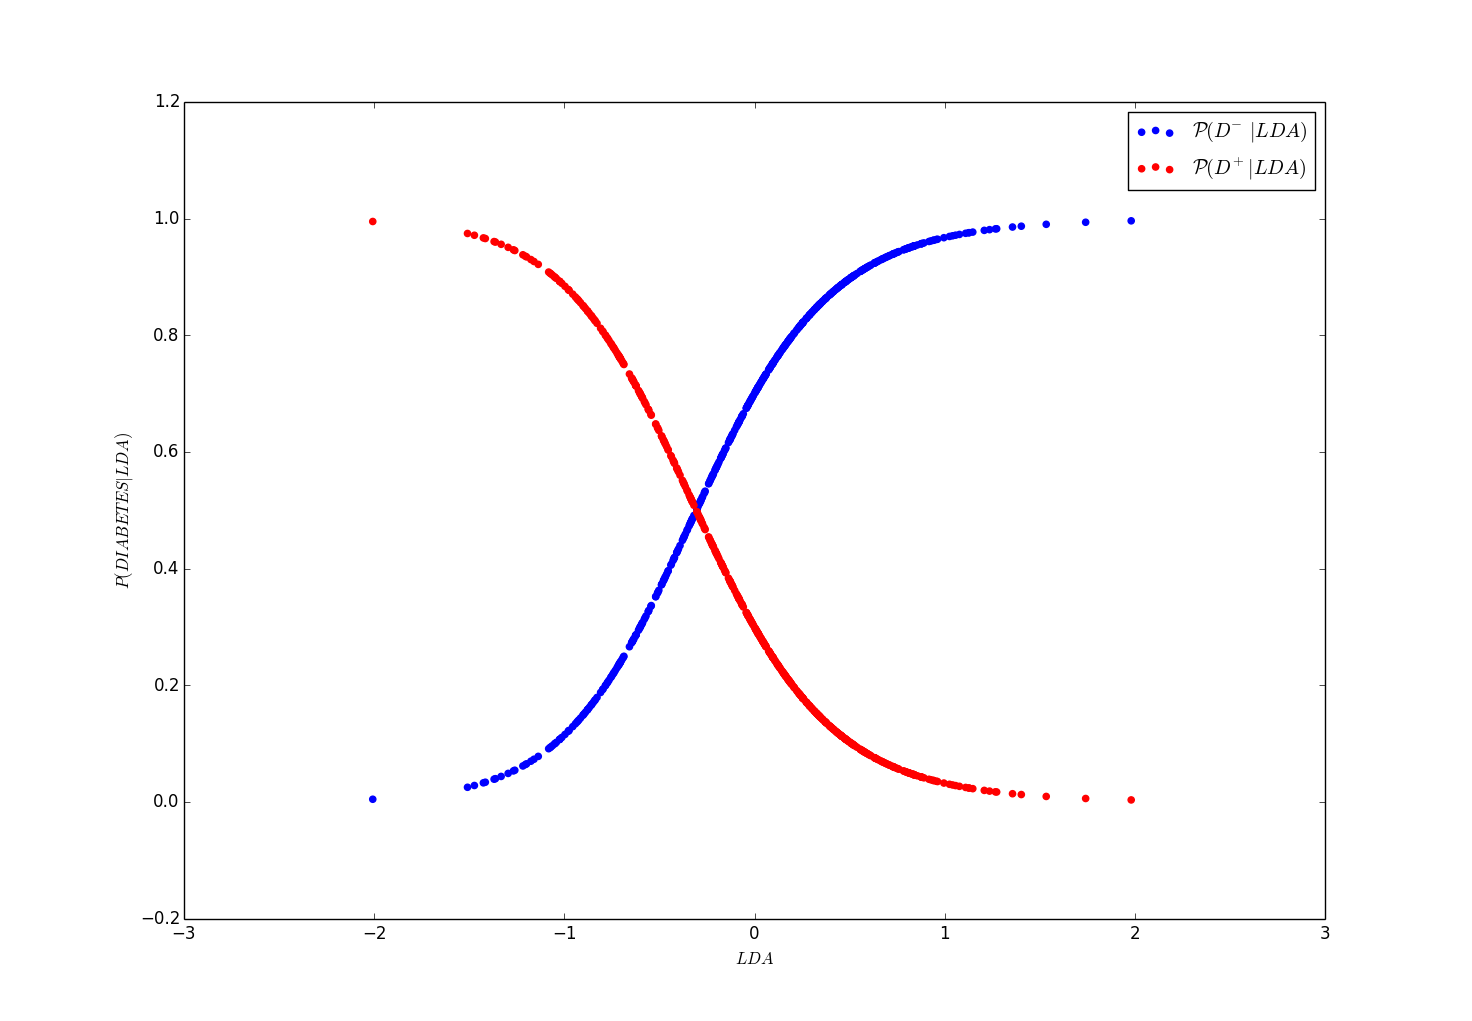
\includegraphics[width=1\linewidth]{images/CP_D8}
        \captionof{figure}{Probabilidad condicional de clase para 8-D}
    \end{minipage}

\end{figure}




\end{appendices}


%----------------------------------------------------------------------------------------
%    DOCUMENT END
%----------------------------------------------------------------------------------------

\end{document}